\documentclass[12pt]{../style-files/ociamthesis}
 
\usepackage{amssymb}
\usepackage{titlesec}
\usepackage{amsmath}
\usepackage{float}
\usepackage{graphicx}
\usepackage{caption}
\usepackage{subfig}
\usepackage{xcolor}
\usepackage[section]{placeins}
\usepackage{mathrsfs}
\usepackage{bm}
\usepackage{stmaryrd}
\usepackage{siunitx}
\usepackage{rotating}
\usepackage[utf8]{inputenc}
\usepackage[round]{natbib}
\usepackage{tikz}
\usetikzlibrary{decorations.markings}
\usetikzlibrary{decorations.pathmorphing}

\usepackage{geometry}
 \geometry{
 a4paper,
 left=40mm,
 right=30mm,
 top=30mm,
 bottom=30mm
 }

\definecolor{theblue}{HTML}{0000CD}

% disable this package for printed version
\usepackage[colorlinks=true, linktocpage=true, allcolors=theblue]{hyperref}

\titleformat{\chapter}[display]
  {\bfseries\Large}
  {\filright\MakeUppercase{\chaptertitlename} \Large\thechapter}
  {1ex}
  {}
  [\vspace{1ex} \hrule \vspace{1pt} \hrule]

\newcommand{\adv}{    {\it Adv. Space Res.}} 
\newcommand{\annG}{   {\it Ann. Geophys.}} 
\newcommand{\aap}{    {\it Astron. Astrophys.}}
\newcommand{\aaps}{   {\it Astron. Astrophys. Suppl.}}
\newcommand{\aapr}{   {\it Astron. Astrophys. Rev.}}
\newcommand{\ag}{     {\it Ann. Geophys.}}
\newcommand{\aj}{     {\it Astron. J.}} 
\newcommand{\apj}{    {\it Astrophys. J.}}
\newcommand{\apjl}{   {\it Astrophys. J. Lett.}}
\newcommand{\apss}{   {\it Astrophys. Space Sci.}} 
\newcommand{\cjaa}{   {\it Chin. J. Astron. Astrophys.}} 
\newcommand{\gafd}{   {\it Geophys. Astrophys. Fluid Dyn.}}
\newcommand{\grl}{    {\it Geophys. Res. Lett.}}
\newcommand{\ijga}{   {\it Int. J. Geomagn. Aeron.}}
\newcommand{\jastp}{  {\it J. Atmos. Solar-Terr. Phys.}} 
\newcommand{\jgr}{    {\it J. Geophys. Res.}}
\newcommand{\mnras}{  {\it Mon. Not. Roy. Astron. Soc.}}
\newcommand{\na}{     {\it New Astronomy}}
\newcommand{\nat}{    {\it Nature}}
\newcommand{\pasp}{   {\it Pub. Astron. Soc. Pac.}}
\newcommand{\pasj}{   {\it Pub. Astron. Soc. Japan}}
\newcommand{\pre}{    {\it Phys. Rev. E}}
\newcommand{\solphys}{{\it Solar Phys.}}
\newcommand{\sovast}{ {\it Soviet  Astron.}} 
\newcommand{\ssr}{    {\it Space Sci. Rev.}}
\newcommand{\caa}{    {\it Chinese Astron. Astrohpys.}} 
\newcommand{\apjs}{   {\it Astrophys. J. Suppl.}}

\begin{document}

\baselineskip=18pt

\setcounter{secnumdepth}{3}
\setcounter{tocdepth}{3}

\setcounter{chapter}{3}

\newcommand{\figdir}{../main/figures/chpt-4/} % where figures are stored

\newcommand{\bv}{\mathbf{v}}
\newcommand{\bB}{\mathbf{B}}

%------------------------------------------------------------------------------
\chapter{Asymmetric waveguides - initial value problem}
\label{chap: IVP}
%------------------------------------------------------------------------------

%------------------------------------------------------------------------------
\section{Chapter introduction}
\label{sec: IVP intro}
%------------------------------------------------------------------------------

Eigenmodes are rightfully considered the building blocks of linear oscillations of complex MHD models. They describe how wave power is spatially distributed across a waveguide and define natural oscillation frequencies. However, when solving an MHD wave problem using an EVP approach, such as was used in Chapter~\ref{chap: EVP}, we use a Fourier decomposition in time, so that the eigenmodes have time dependence proportional to $\exp(i\omega t)$. This is a simple time-dependence: a sinusoidal oscillation with frequency $\omega$, and allows a time-independent solution to be found. Whilst this view is useful for understanding the spatial properties of the wave, eigenmodes do not paint the whole picture. A more complete description involves studying the time-evolution by solving the associated IVP.

The IVP approach to MHD wave problems has been utilised by many authors, developing the theory of time-dependant wave phenomena including phase mixing and resonant absorption. They either solve the IVP analytically or numerically. 

\color{red}
Notes:
IVPs useful for:
Damping/resonance: phase mixing, resonant absorption, wave leakage, heating.
Reflection/transmission: propagation from low atmosphere to upper atmosphere.

\cite{sed71} - original method for asymptotic analysis of MHD IVP. Analogy to Landau damping of hot plasma oscillations.
\cite{and_etal07} - spectral measure interpretation, continuous spectrum, leaky modes.
\cite{rud_etal02} - asymptotic analysis of line-tied straight mag flux tube with transition region.
\cite{rud_etal06} - asymptotic analysis of line-tied straight mag flux tube without transition region. Deeper analysis of Riemann surface and singularities.


Numerical results: \cite{ter_etal06}

Physicality of the principle leaky kink mode: \cite{cal03} solved the initial value problem of transverse waves in a cold magnetic flux tube. \cite{rud_etal06} repeated it showing PLK modes are on an unphysical branch of the complex plane (?). Commented on by \cite{cal06} and in return by \cite{rud_etal06b}. Settled (?) by considering numerical solution by \cite{ter_etal07} and analytically by \cite{and_etal07}. So PLK modes are not physical.

Time scales of wave leakage much longer than time scale of resonant absorption \citep{rob19}, but curvature can amplify leakage \citep{sel_etal07}.

\color{black}

The utility of the IVP approach in the present chapter is to determine a time-scale over which collective and coherent asymmetric oscillations can be expected to develop following an initial perturbation of an MHD waveguides. \textcolor{red}{Can leaky modes Perhaps we can also discuss the resonant absorption of asymmetric waves? Shouldn't be too hard to do this on top of what we've already done. Consider an asymmetric slab with continuous monotonic interfaces. Expect the RA to be stronger on one of the sides. Would this have an impact on the propagation direction of the wave? Do leaky modes transport momentum?}

The structure of this chapter is as follows. Leaky waves play a key role in IVPs in MHD waveguides so Section~\ref{sec: IVP leaky} discusses leaky waves in the IVP context. In Section~\ref{sec: IVP int}, we solve the MHD IVP for a interface between two plasmas, correcting several significant errors made in previous research. In Section~\ref{sec: IVP slab}, we solve the MHD IVP for an asymmetric slab.


%------------------------------------------------------------------------------
\section{Leaky waves}
\label{sec: IVP leaky}
%------------------------------------------------------------------------------

Small amplitude MHD waves guided by an isolated plasma inhomogeneity are made up of \textit{trapped} and \textit{leaky} wave components. Trapped waves maintain a constant (when averaged over a period) amplitude through time and are spatially evanescent away from the waveguide. Trapped waves were the subject of the analysis in Chapter~\ref{chap: EVP}. One can then ask whether there can exist any modes with attenuated amplitude through time. Attenuating amplitude means the waves would be losing energy in the direction of propagation. Without any damping mechanism\footnote{The discontinuous Alfv\'{e}n speed profile used in our model avoids resonant absorption and phase mixing and neglecting viscosity avoids viscous damping.}, there is no way for this energy to be converted into heat. The energy is not \textit{lost}, rather, it is \textit{moved}. Energy must be transported orthogonal to the propagation direction.

To see this mathematically, consider the \textit{Poynting flux}, which represents the directional energy flux of a magnetic field. The Poynting flux is defined as $\mathbf{S} = (\mathbf{E} \times \bB)/\mu_0$ (see, for example, \citealp{pri14}). In ideal MHD, Ohm's law tells us that the electric field is approximately $\mathbf{E} = -(\bv \times \bB)$. Therefore, using a standard vector calculus identity, the Poynting flux can be written as $\mathbf{S} = [B^2\bv - (\bv \cdot \bB)\bB] / \mu_0$. Under the assumption that that wave is temporally attenuating, the angular frequency must have a (negative) imaginary part, $\omega = \omega_R + i\omega_I$. The time-averaged Poynting flux over a wave period, $T = 2\pi/\omega_R$, is a more instructive quantity because it neglects the small changes in energy flux that do not contribute to the energy flux over time-scales longer than a wave period. The velocity perturbation time-averaged from an initial time $t_0$ is
\begin{align}
	\langle \bv \rangle &= \frac{1}{T} \int_{t_0}^{t_0 + T} \bv ~dt \\
	&= \frac{1}{T} \int_{t_0}^{t_0 + T} \mathbf{\hat{v}} e^{i(kz - \omega t)} ~dt \\
	&= \frac{i}{\omega T} \mathbf{\hat{v}} e^{i(kz - \omega t_0)} (e^{\omega_I T} - 1).
\end{align}
To linear order, the time-averaged Poynting flux due to an MHD wave in our model is
\begin{align}
\langle \mathbf{S} \rangle &= \frac{1}{\mu_0}[B_0^2\langle\bv\rangle - (\langle\bv\rangle \cdot \bB_0)\bB_0] \\
&= \frac{iB_0^2}{\omega T \mu_0} \hat{v}_x e^{i(kz - \omega t_0)} (e^{\omega_I T} - 1) \mathbf{\hat{x}}.
\end{align}
For trapped waves, the frequency is purely real, \textit{i.e.} $\omega_I = 0$, hence $\langle \bv \rangle = \mathbf{0}$, giving a vanishing time-averaged Poynting flux (to linear order). For non-trapped waves, the time-averaged Poynting flux is in the transverse direction, orthogonal to the direction of propagation. Energy leaks away from the waveguide, balancing the amplitude attenuation. Waves of this type are known as \textit{leaky}.

As discussed in Chapter~\ref{chpt: ray}, wave leakage can occur for incidence angles greater then the critical angle for total internal reflection. A proportion of the energy is transmitted into the external plasma. When posed as an eigenvalue problem, the leaky modes have eigenfunctions that are spatially oscillatory in the external plasma (Figure~\ref{fig: leaky eigenfunction}) as opposed to trapped modes, which have eigenfunctions that are evanescent in the external plasma (Figure~\ref{fig: trapped eigenfunction}).
\begin{figure}
	\subfloat[Trapped]{
		\includegraphics[width=\textwidth]{\figdir trapped.pdf}
		\label{fig: trapped eigenfunction}
	} \\
	\subfloat[Leaky]{
		\includegraphics[width=\textwidth]{\figdir leaky.pdf}
		\label{fig: leaky eigenfunction}
	}
	\caption{Typical eigenfunctions for trapped and leaky modes of an MHD waveguide. The arrows denote the direction of energy flux.}
	\label{fig: eigenfunction}
\end{figure}
Leaky modes are not normal eigenmodes of the true sense, in that they do not make up any orthogonal set of elements of the MHD Hilbert space. This is equivalent to the frequencies of leaky modes not being elements of the discrete spectrum\footnote{The spectrum of a bounded operator on a Hilbert space is the set of scalars $\omega$ such that the operator $\mathbf{F} - \lambda\mathbf{I}$ does not have a bounded inverse on the Hilbert space. Here, $\mathbf{F}$ and $\mathbf{I}$ are the ideal MHD force operator and the identity operator, respectively. The discrete spectrum is made up of the eigenvalue of the operator $\mathbf{F}$. The spectrum is a generalisation of the set of eigenvalues of an operator in the sense that the discrete spectrum is a subset of the spectrum.}. This is clearly seen by the fact that they perturb plasma at an arbitrary distance from the waveguide, therefore input an infinite amount of energy on the plasma. Instead, they contribute to the continuous spectrum\footnote{The continuous spectrum is the subset of the spectrum whose elements $\lambda$ are dense and that $\mathbf{F} - \lambda\mathbf{I}$ is injective but not surjective.}. For the slab waveguide, the spectral measure associated with the continuous spectrum has peaks at specific frequencies. These peaks are the allowed frequencies of the leaky modes. This gives the erroneous impression that they contribute to the discrete spectrum. Leaky modes of a slab waveguide are analysed in more detail from the perspective of spectral theory by \cite{and_etal07}.

The physical nature of leaky modes is that they dominate to the time-dependent solution for intermediate time scales, \textit{i.e.} much longer than the period of the dominant eigenmode and less than (or of the order of) the timescale of damping due to energy leakage, and intermediate length scales from the waveguide \citep{rud_etal06b,rud_etal02}. This means that they contribute a finite amount of energy, rather than an infinite amount if they were superposed as a standard eigenmode. \textcolor{red}{Maybe say that this has only been shown for tube, we will show it for slab. Only include this if we actually do show it.}


%------------------------------------------------------------------------------
\section{Tangential interface}
\label{sec: IVP int}
%------------------------------------------------------------------------------

In seminal research, and one of the earlier uses of the IVP approach to an MHD wave problem, \cite{rae_etal81} modelled surface waves propagating along an isolated tangential interface, parallel to the $z$-axis, separating two distinct plasmas. In this section, we bring to attention several ways in which the derivation and results of that paper are incorrect and correct the analysis. To our knowledge, this is the first time these errors has been reported.

Consider a stationary, inviscid plasma that is stratified in the $x$-direction only that has unidirectional magnetic field $\bB = (0, 0, B(x))$. Following \cite{rae_etal81}, we let the plasma be incompressible. First, taking Fourier components in the $z$-direction\footnote{To maintain consistency with the remainder of this thesis, we look for parameters proportional to $e^{ikz}$ instead of $e^{-ikz}$ as was taken by \cite{rae_etal81}.}
\begin{equation}
v_x(x,y,z,t) = \hat{v}_x(x,t)e^{ikz},
\end{equation}
the linearised ideal incompressible MHD equations can be simplified to a single equation for the transverse velocity perturbation, namely \citep{pri14}
\begin{equation}
\frac{\partial}{\partial x}\left\{\rho_0\left(\frac{\partial^2}{\partial t^2} + k^2v_A^2\right) \frac{\partial\hat{v}_x}{\partial x}\right\} - k^2\rho_0\left(\frac{\partial^2}{\partial t^2} + k^2v_A^2\right)\hat{v}_x = 0.
\label{gov fourier}
\end{equation}
Next, we take the Laplace transform\footnote{The choice of Laplace transform convention is discussed in Appendix~\ref{app: laplace trans}.}, of this equation, where we define
\begin{equation}
\tilde{v}_x(x) = \mathcal{L}\{\hat{v}_x(x,t)\} = \int_0^\infty \hat{v}_x(x,t)e^{i\omega t} dt.
\end{equation}
Firstly,
\begin{align}
\mathcal{L}\left\{\frac{\partial^2 \hat{v}_x}{\partial t^2}\right\} & = \left[\dot{\hat{v}}_x e^{i\omega t}\right]_0^\infty - i\omega \int_0^\infty \dot{\hat{v}}_x e^{i\omega t} dt \\
& = -\dot{\hat{v}}_{x0} - i\omega\left[\hat{v}_x e^{i\omega t}\right]_0^\infty -\omega^2 \int_0^\infty \hat{v}_x e^{i\omega t} dt \\
& = i\omega \hat{v}_{x0} - \dot{\hat{v}}_{x0} - \omega^2 \tilde{v}_x,
\end{align}
where $\dot{\hat{v}}_x = \partial\hat{v}_x/\partial t$, and we have used the assumption that $\lim_{t \to \infty} \dot{\hat{v}}_{x}(x,t) = \lim_{t \to \infty} \hat{v}_{x}(x,t) = 0$, for all $x$. Therefore, Equation~\eqref{gov fourier} becomes
\begin{align}
\frac{d}{dx} &\left[\rho_0\left(\left\{i\omega \hat{v}_{x0}' - \dot{\hat{v}}_{x0}' - \omega^2\tilde{v}_x'\right\} + k^2v_A^2 \tilde{v}_x'\right)\right] \notag \\
&- k^2\rho_0 \left(\left\{i\omega \hat{v}_{x0} - \dot{\hat{v}}_{x0} - \omega^2\tilde{v}_x\right\} + k^2v_A^2 \tilde{v}_x\right) = 0, \notag
\end{align}
where $\tilde{v}'_x = \partial\tilde{v}_x/\partial x$. By defining $\epsilon = \epsilon(x) = \rho_0(x)(k^2v_A(x)^2 - \omega^2)$, this equation is equivalent to
\begin{align}
\frac{d}{dx} \left[\epsilon \tilde{v}_x'\right] - k^2\epsilon \tilde{v}_x & = - \rho_0 k^2\left(\dot{\hat{v}}_{x0} - i\omega\hat{v}_{x0}\right) + \frac{\partial}{\partial x}\left[\rho_0\left(\dot{\hat{v}}_{x0}' - i\omega\hat{v}_{x0}'\right)\right] \notag \\
& = - \rho_0 k^2\left(\dot{\hat{v}}_{x0} - i\omega\hat{v}_{x0}\right) + \rho_0\left(\dot{\hat{v}}_{x0}'' - i\omega\hat{v}_{x0}''\right) + \frac{d\rho_0}{dx}\left(\dot{\hat{v}}_{x0}' - i\omega\hat{v}_{x0}'\right) \notag \\
& = \rho_0\left[\left(\dot{\hat{v}}_{x0}'' - k^2\dot{\hat{v}}_{x0}\right) - i\omega\left(\hat{v}_{x0}'' - k^2\hat{v}_{x0}\right)\right] + \frac{d\rho_0}{dx}\left(\dot{\hat{v}}_{x0}' - i\omega\hat{v}_{x0}'\right)
\label{gov reduced}
\end{align}
Two equations that will help simplify this equation are derived from the assumption of incompressibility and the definition of vorticity:
\begin{itemize}
	\item $\nabla\cdot\mathbf{v} = 0$, from which it follows that $\hat{v}_x' = -ik \hat{v}_z$.
	\item The vorticity, defined by $\Omega(\mathbf{x},t)\mathbf{\hat{y}} = \hat{\Omega}(x,t)e^{ikz}\mathbf{\hat{y}} = \nabla \times \mathbf{v}(\mathbf{x},t)$, is given by	\begin{equation}
	\hat{\Omega}(x,t) = -\frac{i}{k}\left(\hat{v}''_x - k^2 \hat{v}_x\right).
	\end{equation}
\end{itemize}
Using the above two equations, Equation~\eqref{gov reduced} simplifies to
\begin{equation}
\frac{d}{dx} \left[\epsilon \frac{d \tilde{v}_x}{d x}\right] - k^2\epsilon \tilde{v}_x = f(x), \label{gov}
\end{equation}
where
\begin{equation}f(x) = ik\left\{\rho_0\left[\dot{\hat{\Omega}}_0 - i\omega\hat{\Omega}_0\right] \textcolor{red}{-} \frac{d\rho_0}{dx}\left(\dot{\hat{v}}_{z0} - i\omega\hat{v}_{\textcolor{red}{z}0}\right)\right\}.
\end{equation}
This function is the corrected version of Equations~(11)-(13) of \cite{rae_etal81}. The red opperator is the corrected version. However, because \cite{rae_etal81} assumed that $\partial \rho_0 / \partial x = 0$, this error was inconsequential. Additionally, a typographical error was made in the above equation, where they wrote subscript $x$ in place of our subscript $\textcolor{red}{z}$. Note that there is a factor of -1 discrepency between this function and that of \cite{rae_etal81} due to taking different Fourier forms.

For future utility, we define $\Psi_0 = \Psi(x, 0)$ by function $\Psi(x, t) = k[\rho_0\hat{\Omega}(x, t) - \rho_0'\hat{v}_z(x, t)]$ so that $f(x, \omega) = \omega \Psi_0 + i\frac{\partial \Psi_0}{\partial t}$.


\subsection{Discontinuous interface}

Consider the equilibrium structuring of this plasma with magnetic field and density profiles given by
\begin{equation}
B(x)=
\begin{cases}
B_- & \text{for  }x<0, \\
B_+ & \text{for  }x>0,
\end{cases}
\quad \text{and} \quad
\rho(x)=
\begin{cases}
\rho_- & \text{for  }x<0, \\
\rho_+ & \text{for  }x>0, \\
\end{cases}
\end{equation}
where $B_j$ and $\rho_j$ are uniform for $j = -, +$. In this equilibrium, Equation~\eqref{gov} tells us that transverse velocity perturbation is related to initial perturbations by
\begin{equation}
\frac{d^2\tilde{v}_x}{dx^2} - k^2\tilde{v}_x = 
\begin{cases}
f(x)/\epsilon_-, & \text{for  } x < 0,\\
f(x)/\epsilon_+, & \text{for  } x > 0,
\end{cases}
\label{ivp interface gov}
\end{equation}
and satisfies the boundary conditions
\begin{equation}
\lim_{x \to -\infty}\tilde{v}_x(x) = \lim_{x \to \infty}\tilde{v}_x(x) = 0 \text{ and } \lim_{x \to 0^-}\tilde{v}_x(x) = \lim_{x \to 0^+}\tilde{v}_x(x).
\label{ivp interface BC}
\end{equation}
These boundary conditions correspond to plasma far from the interface being unaffected by its oscillation and that the plasma at the interface remains connected. The second of these is referred to as the \textit{kinematic boundary condition} for a free surface in fluid mechanics \citep{goe_etal04}.

The problem given by Equation~\eqref{ivp interface gov} with boundary conditions~\eqref{ivp interface BC} is a \textit{Sturm-Liouville problem} \citep{boy_etal12}. Sturm-Liouville theory tells us that the Green's function, $G(x; s)$, corresponding to Equation~\eqref{ivp interface gov} must satisfy 
\begin{equation}
\frac{\partial^2G}{\partial x^2} - k^2 G = \delta(x-s), \quad G(-\infty; s) = G(\infty; s) = 0,
\end{equation}
where $\delta$ denotes the Dirac Delta function. It is instructive to piecewise define the Green's function as
\begin{equation}
G(x; s) = 
\begin{cases}
G_-(x; s), & \text{for } x < 0, \\
G_+(x; s), & \text{for } x > 0.
\end{cases}
\end{equation}
The general solution of the equation for $G_-$ for $x < 0$ is
\begin{equation}
G_-(x; s) = c_1e^{kx} + c_2e^{-kx},
\end{equation}
where $c_1$ and $c_2$ are constants with $c_2 = 0$ for $x < s$ and $c_1 = 0$ for $x > s$. Ensuring $G_-$ and $\partial G_- / \partial x$ have jumps of 0 and 1 at $x = s$, respectively, determines $c_1$ and $c_2$, so that $G_-(x;s)$ is
\begin{equation}
\begin{aligned}
G_-(x; s) & = -\frac{1}{2k} 
\begin{cases}
e^{kx}e^{-ks}, & \text{for } -\infty < x < s, \\
e^{-kx}e^{ks}, & \text{for } s< x < 0,
\end{cases} \\
& = - \frac{1}{2k}\left[e^{ks}e^{-kx}H(x-s) + e^{-ks}e^{kx}H(s-x)\right],
\end{aligned}
\end{equation}
The Sturm-Liouville problem for each plasma ($x < 0$ and $x > 0$) has an inhomogeneous boundary condition at the interface. Therefore, we must add to the standard Green's function solution a term that is a solution to the homogeneous equation with inhomogeneous boundary conditions. In this manner, we find that the solution for $x < 0$ is
\begin{equation}
\tilde{v}_x(x) = \tilde{A}_-e^{kx} \textcolor{red}{+} \frac{1}{\epsilon_-}\int_{-\infty}^{0} G(x; s) f(s) ds. \label{sol -}
\end{equation}
Similarly, the solution for $x > 0$ is
\begin{equation}
\tilde{v}_x(x) = \tilde{A}_+e^{-kx} + \frac{1}{\epsilon_+}\int_{0}^{\infty} G(x; s) f(s) ds. \label{sol +}
\end{equation}
where
\begin{equation}
G(x; s) = - \frac{1}{2k}\left[e^{ks}e^{-kx}H(x-s) + e^{-ks}e^{kx}H(s-x)\right].
\end{equation}
Equation~\eqref{sol -} is the corrected version of Equation~(16) in \cite{rae_etal81}. In \cite{rae_etal81}, they have a - instead of a +. We explicitly demonstrate the error in their solution in Appendix~\ref{app: error}.

By imposing continuity of transverse velocity perturbation, we can determine the constants $A_-$ and $A_+$ to be
\begin{align}
\tilde{A}_+ & = \frac{1}{k(\epsilon_- + \epsilon_+)}\left[\textcolor{red}{-} \: \int_{-\infty}^0 f(s)e^{ks} ds - \frac{1}{2}\left(1 - \frac{\epsilon_-}{\epsilon_+}\right)\int_0^\infty f(s)e^{-ks} ds\right], \\
\tilde{A}_- & = \frac{1}{k(\epsilon_- + \epsilon_+)}\left[-\int_0^\infty f(s)e^{-ks} ds \: \textcolor{red}{-} \: \frac{1}{2}\left(1 - \frac{\epsilon_+}{\epsilon_-}\right)\int_{-\infty}^0 f(s)e^{ks} ds\right],
\end{align}
which differs to that given by \cite{rae_etal81} by the red operators.

The solution in time is found by taking the inverse Laplace transform of Equations~\eqref{sol -} and~\eqref{sol +}. This is not possible for arbitrary initial conditions. To demonstrate where the corrected version deviated from the errors made in \cite{rae_etal81}, we derive the solution for several specific initial conditions.


\subsubsection{Solution for specific initial conditions}

The errors in the solution given above lead to errors in the specific solutions to the initial value problem. The corrected solutions for specific initial conditions used by \cite{rae_etal81} are given below:

\begin{enumerate}
	\item \label{IC1} \textit{Vorticity constant everywhere at $t = 0$}. When the initial vorticity is constant with respect to $x$, \textit{i.e.} $\Omega(x,0) = \Omega_0$, Equation~\eqref{ivp interface sol correct} gives
	\begin{equation}
	\tilde{v}_x = -\frac{\rho_0\omega\Omega_0}{k}
	\begin{cases}
	\left(1 + \frac{\epsilon_- - \epsilon_+}{\epsilon_- + \epsilon_+}e^{kx}\right)/\epsilon_-, & \text{for } x<0, \\
	\left(1 + \frac{\epsilon_+ - \epsilon_-}{\epsilon_- + \epsilon_+}e^{-kx}\right)/\epsilon_+, & \text{for } x>0.
	\end{cases}
	\end{equation}
	\item \label{IC2} \textit{Step function vorticity at $t = 0$}. When the initial vorticity is given by $\Omega(x,0) = \Omega_0H(-x)$, Equation~\eqref{ivp interface sol correct} gives
	\begin{equation}
	\tilde{v}_x = -\frac{\rho_0\omega\Omega_0}{k}
	\begin{cases}
	\left(1 - \frac{\epsilon_+}{\epsilon_- + \epsilon_+}e^{kx}\right)/\epsilon_-, & \text{for } x<0, \\
	\frac{1}{\epsilon_- + \epsilon_+}e^{-kx}, & \text{for } x>0.
	\end{cases}
	\end{equation}
	\item  \label{IC3} \textit{Impulsive vorticity at $t = 0$}. When the initial vorticity\footnote{Note that \cite{rae_etal81} incorrectly use the impulsive initial condition $\Omega(x,0) = \Omega_0\delta(x-x_0)$. This can be shown to be erroneous by considering that the dimensions of the left-hand side, $\Omega(x,0)$, are $[\mathrm{Time}^{-1}]$ and therefore not equal to the dimensions of the right-hand side, $\Omega_0\delta(x-x_0)$, namely $[\mathrm{Distance}^{-1}\mathrm{Time}^{-1}]$. They also omit, without explanation, the density, $\rho_0$, from their solutions.} is given by {$\Omega(x,0) = \Omega_0\delta(k(x-x_0))$}, for $x_0>0$, Equation~\eqref{ivp interface sol correct} gives
	\begin{equation}
	\tilde{v}_x = -\frac{\rho_0\omega\Omega_0}{k}
	\begin{cases}
	\frac{1}{\epsilon_- + \epsilon_+}e^{-k(x_0 - x)}, & \text{for } x < 0, \\
	\frac{\epsilon_+ - \epsilon_-}{2\epsilon_+(\epsilon_- + \epsilon_+)}e^{-k(x + x_0)} + \frac{e^{-k(x_0 - x)}}{2\epsilon_+}, & \text{for } 0<x<x_0, \\
	\frac{\epsilon_+ - \epsilon_-}{2\epsilon_+(\epsilon_- + \epsilon_+)}e^{-k(x + x_0)} + \frac{e^{-k(x - x_0)}}{2\epsilon_+}, & \text{for } x>x_0.
	\end{cases}
	\end{equation}
\end{enumerate}
%
\begin{figure}
	\includegraphics[width=\textwidth]{\figdir v_x.png}
	\caption{Original \cite{rae_etal81} (blue) and corrected (green) solutions for the velocity perturbation, $\tilde{v}_x$, for initial condition~\ref{IC1} (left),~\ref{IC2} (middle), and~\ref{IC3} (right). The blue and green curved are the same in the right panel.}
	\label{fig: vx}
\end{figure}
Figure~\ref{fig: vx} illustrates the solutions for the transverse velocity perturbation, $\tilde{v}_x$, for the three specific initial conditions given above, showing both the original and corrected initial transverse velocities.

The full solution for the transverse velocity, $v_x(x, z, t) = \hat{v}_x(x,t)e^{ikz}$ is found by taking the inverse Laplace transform of $\tilde{v}_x$, such that
\begin{equation}
\hat{v}_x(x,t) = \frac{1}{2\pi} \lim_{T \to \infty} \int_{-T+ i\gamma}^{T + i\gamma} \tilde{v}_x(x)e^{-i\omega t} d\omega,
\end{equation}
where $\gamma$ is real and such that all the singularities of the integrand lie below the contour of integration in the complex plane. Using Cauchy's Residue Theorem, it follows that
\begin{equation}
\hat{v}_x(x, t) = -i\sum \mathrm{Res}\left\{\tilde{v}_xe^{-i\omega t}\right\},
\end{equation}
where the summation is over all the singularities of the argument.

Considering initial condition~\ref{IC1}, with uniform vorticity, the singularities of this function occur at $\epsilon_- = 0$, $\epsilon_+ = 0$, and $\epsilon_- + \epsilon_+ = 0$. This corresponds to simple poles at $\omega = \pm kv_{A-}$, $\omega = \pm kv_{A+}$, and $\omega = \pm kv_s$, respectively, where
\begin{equation}
v_s = \sqrt{\frac{v_{A-}^2 + v_{A+}^2}{2}}.
\end{equation}
The residues associated to each singularity are
\begin{align}
\mathrm{Res}\left\{\tilde{v}_x e^{-i\omega t}; \pm kv_{A+}\right\} &= \frac{\Omega_0}{2k} e^{\mp ikv_{A+}t}
\begin{cases}
0, & \text{for  } x < 0, \\
1 - e^{-kx}, & \text{for  } x > 0, 
\end{cases} \\
\mathrm{Res}\left\{\tilde{v}_x e^{-i\omega t}; \pm kv_{A-}\right\} &= \frac{\Omega_0}{2k} e^{\mp ikv_{A-}t}
\begin{cases}
1 - e^{kx}, & \text{for  } x < 0, \\
0, & \text{for  } x > 0,
\end{cases} \\
\mathrm{Res}\left\{\tilde{v}_x e^{-i\omega t}; \pm kv_{s}\right\} &= \frac{\Omega_0}{2k} e^{\mp ikv_st} 
\begin{cases}
e^{kx}, & \text{for  } x < 0, \\
e^{-kx}, & \text{for  } x > 0.
\end{cases}
\end{align}
By summing these residues, we find that
\begin{equation}
\hat{v}_x(x, t) = -\frac{i\Omega_0}{k} \begin{cases}
\cos(kv_{A-}t)\left(1-e^{kx}\right) + \cos(kv_st)e^{kx}, & \text{for  } x<0, \\
\cos(kv_{A+}t)\left(1-e^{-kx}\right) + \cos(kv_st)e^{-kx}, & \text{for  } x>0. \\
\end{cases}
\label{sol int}
\end{equation}
This solution differs from that given by \cite{rae_etal81} most notably with a contribution from surface waves (second term), not just body waves (first term).

The full solution for $v_x$, when the initial disturbance is of the form of a single wave, is recovered by multiplying the above expression by $e^{ikz}$. In reality, an initial disturbance will be of finite extent. This is the subject of the following subsection.


\subsubsection{Solution for an initial disturbance of finite extent}

The response to a disturbance of finite extent is obtained by a superposition over the wavenumber $k$, that is
\begin{equation}
v_x(x, z, t) = \frac{1}{2\pi}\int_{-\infty}^{\infty} \hat{v}_x(x, t) e^{ikz} ~dz.
\end{equation}
This is the inverse Fourier transform.

Let's consider an initial impulse that has uniform vorticity with respect to $x$ and is uniform over a finite range $[-z_0, z_0]$, outside of which it is zero. Precisely, the initial velocity is
\begin{equation}
v_x(x, z, 0) = \frac{v_0}{2z_0}\left[H(z + z_0) - H(z - z_0)\right],
\end{equation}
where $H$ is the Heaviside step function and $v_0$ is constant. The division by $2z_0$ ensures invariance of the integral of the initial velocity as the domain of initial disturbance is varied. In particular, it means that in the limit as $z_0 \to 0$, the initial velocity is a Dirac Delta pulse. Therefore, the initial vorticity is
\begin{equation}
\Omega(x, z, 0) \mathbf{\hat{y}} = \nabla \times \bv = \frac{v_0}{2z_0}\left[\delta(z + z_0) - \delta(z - z_0)\right] \mathbf{\hat{y}},
\end{equation}
which, in $k$-space, is
\begin{equation}
\hat{\Omega}(x, 0) = \int_{-\infty}^{\infty} \Omega(x, z, 0) e^{-ikz} ~dz = i\frac{v_0}{z_0}\sin(kz_0).
\end{equation}
The temporal evolution of this initial velocity pulse over a finite $z$-domain is, for the region $\pm x > 0$,
\begin{align}
v_x(x, z, t) &= -\frac{v_0}{2\pi z_0} \int_{\infty}^{\infty} \frac{1}{k}\sin(kz_0) \left[\left(\cos(kv_{A\pm}t) - \cos(kv_st)\right)e^{-|k||x|} - \cos(kv_{A\pm}t)\right] e^{ikz} ~dk \\
& = -\frac{v_0}{\pi z_0} \int_{0}^{\infty} \frac{1}{k} \left[\sin(k(z + z_0)) - \sin(k(z - z_0))\right] \left[(\cos(kv_{A\pm}t) - \cos(kv_st))e^{-k|x|} - \cos(kv_{A\pm}t)\right] ~dk,
\end{align}
where we have used the fact that an odd function integrated over the real line in zero and an even function integrated over the real line is twice its integral over the positive real line. We also used the product-to-sum identity $2\cos{\theta}\sin{\phi} = \sin(\theta + \phi) - \sin(\theta - \phi)$. Further, by use of the similar identity $2\sin{\theta}\cos{\phi} = \sin(\theta + \phi) + \sin(\theta - \phi)$, we are reduce to a series of integrals like
\begin{equation}
\int_{0}^{\infty} \frac{1}{k}\sin(k(z + z_0 + v_{A\pm}))e^{-k|x|} ~dk,
\end{equation}
and
\begin{equation}
\int_{0}^{\infty} \frac{1}{k}\sin(k(z + z_0 + v_{A\pm})) ~dk.
\end{equation}
Both of these are known integrals (see, for example, \citealp{abr_etal65}). The general form of the first integral can be evaluated like
\begin{equation}
\int_{0}^{\infty} \frac{1}{x}\sin(ax) e^{-bx} ~dx = \tan^{-1}\left(\frac{a}{b}\right),
\end{equation}
for $b > 0$. The second of these is a limiting case of the \textit{sine integral}, $\mathrm{Si}(x)$, which can be evaluated in its general form as
\begin{align}
\int_{0}^{\infty} \frac{1}{t}\sin(at) ~dt &= \lim_{x \to \infty}\int_{0}^{ax} \frac{1}{t}\sin{t} ~dt \\
&= \lim_{x \to \infty} \mathrm{Si}(ax)  \\
&=
\begin{cases}
-\pi/2, &\text{if  } a < 0, \\
0, &\text{if  } a = 0, \\
\pi/2, &\text{if  } a > 0,
\end{cases} \\
&= \frac{\pi}{2} \left[2H(a) - 1\right].
\end{align}
Using the above results leads us to the solution
\begin{align}
v_x(x, z, t) = \frac{v_0}{4\pi z_0} \bigg[ &-\tan^{-1}\left( \frac{z + z_0 + v_{A\pm}t}{|x|} \right) - \tan^{-1}\left( \frac{z + z_0 - v_{A\pm}t}{|x|} \right)  \notag \\
&+ \tan^{-1}\left( \frac{z - z_0 + v_{A\pm}t}{|x|} \right) + \tan^{-1}\left( \frac{z - z_0 - v_{A\pm}t}{|x|} \right) \notag \\
&+ \tan^{-1}\left( \frac{z + z_0 + v_st}{|x|} \right) + \tan^{-1}\left( \frac{z + z_0 - v_st}{|x|} \right) \notag \\
&- \tan^{-1}\left( \frac{z - z_0 + v_st}{|x|} \right) - \tan^{-1}\left( \frac{z - z_0 - v_st}{|x|} \right) \notag \\
&+ \pi \left\{ H(z + z_0 + v_{A\pm}t) + H(z + z_0 - v_{A\pm}t) \right.  \notag \\
&\left. - H(z - z_0 + v_{A\pm}t) - H(z - z_0 - v_{A\pm}t) \right\} \bigg], \label{sol top hat}
\end{align}
The solution given by Equation~\eqref{sol top hat} corresponds to surface waves and body waves with corresponding wakes that propagate at characteristic speeds $v_s$ and $v_{A\pm}$, where the $\pm$ refers to the side of the interface. By taking $t = 0$ in Equation~\eqref{sol top hat}, the initial velocity profile is recovered. In the limit as $z_0 \to \infty$, we find that the temporal evolution of the initial velocity pulse $v_x(x, z, 0) = v_0 \delta(z)$ is
\begin{align}
v_x(x, z, t) = \frac{v_0}{2\pi} \bigg[ &- \frac{|x|}{x^2 + (z + v_{A\pm}t)^2} - \frac{|x|}{x^2 + (z - v_{A\pm}t)^2} \notag \\
&+ \frac{|x|}{x^2 + (z + v_st)^2} + \frac{|x|}{x^2 + (z - v_st)^2} \notag \\
&+ \pi\{\delta(z + v_{A\pm}t) + \delta(z - v_{A\pm}t)\} \bigg]. \label{sol dirac delta}
\end{align}
In deriving the above limit we have used the results that, by definition of the Dirac Delta function,
\begin{equation}
\lim_{z_0 \to 0} \left[\frac{1}{2z_0} \left\{H(z + z_0) - H(z - z_0)\right\}\right] = \delta(z),
\end{equation}
and, by L'Hopital's rule,
\begin{align}
&\lim_{z_0 \to 0} \left[\frac{1}{2z_0}\left\{\tan^{-1}\left( \frac{z + z_0 + v_{A\pm}t}{|x|} \right) - \tan^{-1}\left( \frac{z - z_0 + v_{A\pm}t}{|x|} \right)\right\}\right] \\
&= \frac{1}{2} \lim_{z_0 \to 0} \frac{d}{dz_0} \left[\tan^{-1}\left( \frac{z + z_0 + v_{A\pm}t}{|x|} \right) - \tan^{-1}\left( \frac{z - z_0 + v_{A\pm}t}{|x|} \right)\right] \\
&= \frac{1}{2} \lim_{z_0 \to 0} \left[ \frac{|x|}{x^2 + (z + z_0 + v_{A\pm}t)^2} + \frac{|x|}{x^2 + (z - z_0 + v_{A\pm}t)^2} \right] \\
&= \frac{|x|}{x^2 + (z + v_{A\pm}t)^2}.
\end{align}
Equation~\eqref{sol dirac delta}, where we can see the contribution from the surface mode as well as the body mode, is the corrected version of Equation~(34) in \cite{rae_etal81}.






\color{red}
\subsection{Continuous interface}
\color{black}




































%------------------------------------------------------------------------------
\section{Asymmetric slab}
\label{sec: IVP slab}
%------------------------------------------------------------------------------

\textcolor{red}{Calculate leaky mode frequencies using EVP approach?}

\subsection{Incompressible}

Consider equilibrium magnetic field and density profiles given by
\begin{equation}
B(x)=
\begin{cases}
B_1, & \text{if  }x<-x_0, \\
B_0, & \text{if }|x|\leq{x_0}, \\
B_2, & \text{if  }x>x_0,
\end{cases}
\quad \text{and} \quad
\rho(x)=
\begin{cases}
\rho_1, & \text{if  }x<-x_0, \\
\rho_0, & \text{if }|x|\leq{x_0}, \\
\rho_2, & \text{if  }x>x_0,
\end{cases}
\end{equation}
Perturbation to the transverse velocity perturbations are related to initial perturbations of this equilibrium by
\begin{equation}
\frac{d^2\tilde{v}_x}{dx^2} - k^2\tilde{v}_x = 
\begin{cases}
f(x, \omega)/\epsilon_1, & \text{if  } x<-x_0,\\
f(x, \omega)/\epsilon_0, & \text{if  } |x|<x_0,\\
f(x, \omega)/\epsilon_2, & \text{if  } x>x_0,
\end{cases}
\label{ivp gov slab 2}
\end{equation}
under the boundary conditions
\begin{equation}
\lim_{x \to -\infty}\tilde{v}_x(x) = \lim_{x \to \infty}\tilde{v}_x(x) = 0, \text{ and } \lim_{x \to \pm x_0^-}\tilde{v}_x(x) = \lim_{x \to \pm x_0^+}\tilde{v}_x(x).
\label{ivp slab BC}
\end{equation}

Sturm-Liouville Theory tells us that the Green's function, $G(x;s)$, corresponding to Equation~\eqref{ivp gov slab 2} must satisfy 
\begin{equation}
\frac{\partial^2G}{\partial x^2} - k^2 G = \delta(x - s), \quad G(-x_0; s) = G(x_0; s) = 0.
\end{equation}
It is instructive to piecewise define the Green's function as
\begin{equation}
G(x; s) = 
\begin{cases}
G_1(x; s), & \text{if } x < -x_0, \\
G_0(x; s), & \text{if } |x| < x_0, \\
G_2(x; s), & \text{if } x_0 < x.
\end{cases}
\end{equation}
The general solution, for $|x| < x_0$, of the equation for $G_0$ is
\begin{equation}
G_0(x; s) = c_1\sinh(k(x - x_0)) + c_2\sinh(k(x + x_0)),
\end{equation}
where $c_1 = 0$ for $x < s$ and $c_2 = 0$ for $x > s$. Ensuring $G_0$ and $\partial G_0 / \partial x$ have jumps of 0 and 1, respectively, at $x = s$  determines $c_1$ and $c_2$, so that $G_0(x;s)$ is
\begin{equation}
G_0(x;s) = \frac{1}{k\sinh(2k x_0)}
\begin{cases}
\sinh(k(s - x_0))\sinh(k(x + x_0)), & \text{if } -x_0<x<s, \\
\sinh(k(x - x_0))\sinh(k(s + x_0)), & \text{if } s<x<x_0.
\end{cases}
\end{equation}

Because the boundary conditions at the interfaces are inhomogeneous, we must add to the standard Green's function solution a term that is a solution to the homogeneous equation and the inhomogeneous boundary conditions. In this manner, we find that the solution within the slab is
\begin{align}
\tilde{v}_x(x) = &\frac{1}{\sinh{2kx_0}} \left[ \tilde{A}_1\sinh(k(x_0 - x)) + \tilde{A}_2\sinh(k(x_0 + x)) \right] \notag \\
&+ \frac{1}{\epsilon_0}\int_{-x_0}^{x_0} G_0(x;s) f(s, \omega) ds,
\label{sol 0}
\end{align}
where $\tilde{A}_1 = \tilde{v}_x(-x_0)$ and $\tilde{A}_2 = \tilde{v}_x(x_0)$.

Similarly, we find that the Green's function for the plasma outside the slab is 
\begin{equation}
G_1(x;s) = \frac{1}{k}
\begin{cases}
e^{k(x + x_0)}\sinh(k(s + x_0)), & \text{if } x < s, \\
e^{k(s + x_0)}\sinh(k(x + x_0)), & \text{if } s < x < -x_0,
\end{cases}
\end{equation}
for $x < -x_0$, and
\begin{equation}
G_2(x;s) = -\frac{1}{k}
\begin{cases}
e^{-k(s - x_0)}\sinh(k(x - x_0)), & \text{if } x_0 < x < s, \\
e^{-k(x - x_0)}\sinh(k(s - x_0)), & \text{if } s < x,
\end{cases}
\end{equation}
for $x > x_0$. Therefore, the solution outside the slab is
\begin{equation}
\tilde{v}_x(x) = \tilde{A}_1e^{k(x_0 + x)} + \frac{1}{\epsilon_1}\int_{-\infty}^{-x_0} G_1(x;s) f(s, \omega) ds,
\label{sol 1}
\end{equation}
for $x < -x_0$, and
\begin{equation}
\tilde{v}_x(x) = \tilde{A}_2e^{k(x_0 - x)} + \frac{1}{\epsilon_2}\int_{x_0}^{\infty} G_2(x;s) f(s, \omega) ds,
\label{sol 2}
\end{equation}
for $x > x_0$.

To establish physically relevant solutions, we require that the transverse velocity and the total pressure are continuous over each interface. The construction of Equations~\eqref{sol 0},~\eqref{sol 1}, and~\eqref{sol 2} ensures that the transverse velocity is automatically continuous over the boundaries. Using Equation~\eqref{tot p}, the perturbation in the total pressure for a compressible plasma is given by $\tilde{p}_T(x) = \Lambda\tilde{v}'_x/m$.
%where
%\begin{equation}
%\Lambda = \frac{i\rho(\omega^2 - k^2v_A^2)}{m\omega},
%\quad
%m^2 = \frac{(k^2v_A^2 - \omega^2)(k^2c_0^2 - \omega^2)}{(c_0^2 + v_A^2)(k^2c_T^2 - \omega^2)},
%\quad \text{and} \quad
%c_T^2 = \frac{c_0^2 v_A^2}{c_0^2 + v_A^2}.
%\end{equation}
When the plasma is incompressible, $m^2 \to k^2$. Therefore, continuity in total pressure is equivalent to continuity in $\epsilon(x)\tilde{v}_x'(x)$ for an incompressible plasma. Applying this boundary condition gives
\begin{equation}
\tilde{A}_1(\omega) = \frac{T_1(\omega)}{k D(\omega)}, \quad \tilde{A}_2(\omega) = \frac{T_2(\omega)}{k D(\omega)},
\end{equation}
where
\begin{equation}
D(\omega) = \epsilon_0 \left(\epsilon_1 + \epsilon_2\right)\cosh(2kx_0) + (\epsilon_0^2 + \epsilon_1\epsilon_2)\sinh(2kx_0)
\label{D incomp}
\end{equation}
is called the \textit{dispersion function} and $T_{1,2}$ are functionals given by
\begin{align}
T_1(\omega) &= T_1[f](\omega) = - (I_0^- + I_1) \left[\epsilon_0\cosh(2kx_0) + \epsilon_2\sinh(2kx_0)\right] - \epsilon_0 \left(I_0^+ + I_2\right), \\
T_2(\omega) &= T_2[f](\omega) = - \epsilon_0\left(I_0^- + I_1\right) - \left(I_0^+ + I_2\right)\left[\epsilon_0\cosh(2kx_0) + \epsilon_1\sinh(2kx_0)\right],
\end{align}
where
\begin{align}
I_0^\pm &= I_0^\pm[f](\omega) = \int_{-x_0}^{x_0} \frac{\sinh(k(x_0 \pm s))}{\sinh(2kx_0)} f(s, \omega) ds, \\
I_1 &= I_1[f](\omega) = \int_{-\infty}^{-x_0} e^{k(x_0 + s)} f(s, \omega) ds, \\
I_2 &= I_2[f](\omega) = \int_{x_0}^\infty e^{k(x_0 - s)} f(s, \omega) ds.
\end{align}


\subsubsection{Solution in time}

To recover the transverse velocity, $v_x(x, t)$, we employ the inverse Laplace transform. We will do this for a general initial perturbation. Focusing firstly on the region $x < -x_0$, the solution is
\newcommand{\e}{\epsilon}
\begin{align}
v_x &= \mathcal{L}^{-1} \left\{ \tilde{A}_1 e^{k(x+x_0)} + \frac{1}{\e_1} \int_{-\infty}^{-x_0} G_1(x;s)f(s, \omega)ds \right\}, \\
&= e^{k(x+x_0)} \mathcal{L}^{-1}\left\{ \tilde{A}_1 \right\} + \int_{-\infty}^{-x_0} G_1(x;s) \mathcal{L}^{-1}\left\{ \frac{f(s, \omega)}{\e_1} \right\} ds, \\
&= e^{k(x+x_0)} \mathcal{L}^{-1}\left\{ \tilde{A}_1 \right\} + \int_{-\infty}^{-x_0} G_1(x;s) \left[ \Psi (s, 0) \mathcal{L}^{-1}\left\{ \frac{\omega}{\e_1} \right\} + i \frac{\partial \Psi}{\partial t}(s, 0) \mathcal{L}^{-1}\left\{ \frac{1}{\e_1} \right\}\right] ds,
\label{sol incomp}
\end{align}
We evaluate each of the three inverse Laplace transforms in turn.

The first inverse Laplace transform,
\begin{equation}
\mathcal{L}^{-1} \{\tilde{A}_1\} = \frac{1}{2\pi} \int_{-\infty + i\gamma}^{\infty + i\gamma} \tilde{A}_1 e^{-i\omega t} ~d\omega,
\end{equation}
is calculated as follows. The functions $\epsilon_{0,1,2}$ are quadratic in $\omega$, and are therefore entire. The integrals $I_{1,2}$ and $I_0^\pm$ are, in general, linear functions of $\omega$ so also contribute no singularities. Therefore, $T_1$ and $T_2$ are entire functions. Hence, the singularities of $\tilde{A}_1$ are precisely the zeros of the dispersion function, $D(\omega)$.

The zeros of $D(\omega)$ are determined by firstly noting that $D=0$ is the dispersion relation of the corresponding eigenvalue problem solved in Chapter~\ref{chap: EVP} and by \cite{zsa_etal18}. To recap, the dispersion relation governing transverse wave propagation parallel to the magnetic field in an asymmetric slab of compressible plasma is given by
\begin{equation}
2(\Lambda_0^2 + \Lambda_1 \Lambda_2) + \Lambda_0(\Lambda_1 + \Lambda_2)[\tanh(m_0x_0) + \coth(m_0x_0)] = 0,
\label{DR}
\end{equation}
where
\begin{equation}
\Lambda_j = -\frac{i\rho_j(k^2v_{Aj}^2 - \omega^2)}{\omega m_j},
\quad
\text{and}
\quad
m_j^2 = \frac{(k^2c_j^2 - \omega^2)(k^2v_{Aj}^2 - \omega^2)}{(c_j^2 + v_{Aj}^2)(k^2c_{Tj}^2 - \omega^2)},
\end{equation}
for $j = 0, 1, 2$. When compressibility is neglected, such that the sound speeds, $c_j$, approach infinity, we have $c_{Tj}^2 \to v_{Aj}^2$, $m_j^2 \to k^2$, and therefore $\Lambda_j = -i\rho_j(k^2v_{Aj}^2 - \omega^2)/\omega k = -i\epsilon_j / \omega k$, for $j=0,1,2$. Therefore, Equation~\eqref{DR} can be reduced to the dispersion relation for an incompressible magnetic slab, which is
\begin{equation}
2\left(\epsilon_0^2 + \epsilon_1 \epsilon_2\right) + \epsilon_0(\epsilon_1 + \epsilon_2)[\tanh(m_0x_0) + \coth(m_0x_0)] = 0.
\end{equation}
This equation can easily to shown to be equivalent to $D(\omega) = 0$, where $D(\omega)$ is given by Equation~\eqref{D incomp}. It follows that the zeros of $D(\omega)$ are precisely the eigenvalues of the asymmetric incompressible magnetic slab. This is a specific case of a powerful general result for initial value problems and their corresponding eigenvalue problems which is explored in the MHD setting by \cite{goe_etal04}, Chapter 10.2.

The zeros of $D$ are found by writing the equation $D(\omega) = 0$ as
\begin{equation}
\epsilon_0(\epsilon_1 + \epsilon_2) + \left(\epsilon_0^2 + \epsilon_1\epsilon_2\right)\tanh(2kx_0) = 0
\end{equation}
and substituting expressions for $\epsilon(x)$, which gives
\begin{align}
&\rho_0\left(k^2v_{A0}^2 - \omega^2\right)\left[\rho_1\left(k^2v_{A1}^2 - \omega^2\right) + \rho_2\left(k^2v_{A2}^2 - \omega^2\right)\right] \notag \\
&+ \left[\rho_0^2\left(k^2v_{A0}^2 - \omega^2\right)^2 + \rho_1\rho_2\left(k^2v_{A1}^2 - \omega^2\right)\left(k^2v_{A2}^2 - \omega^2\right)\right]\tanh(2kx_0) = 0.
\end{align}
The above equation can be rewritten as a quadratic in $(\omega/k)^2$, namely
\begin{equation}
a \left(\frac{\omega}{k}\right)^4 + b \left(\frac{\omega}{k}\right)^2 + c = 0,
\end{equation}
which has solutions
\begin{equation}
\left(\frac{\omega_{0\pm}}{k}\right)^2 = \frac{-b \pm \sqrt{b^2 - 4ac}}{2a},
\end{equation}
where
\begin{align}
a &= \left(\rho_0^2 + \rho_1\rho_2\right)\tanh(2kx_0) + \rho_0(\rho_1 + \rho_2), \label{solution a} \\
b &= -\left(2\rho_0^2v_{A0}^2 + \rho_1\rho_2\left(v_{A1}^2 + v_{A2}^2\right)\right)\tanh(2kx_0) \notag \\
& \quad - \rho_0 \left\{ \rho_1\left(v_{A0}^2 + v_{A1}^2\right) + \rho_2\left(v_{A0}^2 + v_{A2}^2\right) \right\}, \label{solution b} \\
c &= (\rho_0^2v_{A0}^4 + \rho_1\rho_2v_{A1}^2v_{A2}^2)\tanh(2kx_0) + \rho_0v_{A0}^2(\rho_1v_{A1}^2 + \rho_2v_{A2}^2). \label{solution c}
\end{align}
The solutions, $\pm\omega_{0\pm}$, must be real \citep{goe_etal04}. Additionally, the solutions corroborate with the corresponding incompressible eigenfrequencies for an interface and a symmetric slab, shown in Appendices~\ref{app: interface} and~\ref{app: symmetric}, respectively.

\textcolor{red}{
The zeroes of the dispersion function, that is, the normal modes, make up the discrete spectrum of modes. In general, the governing MHD wave equation contains a continuous spectrum in addition to the discrete spectrum. The continuous spectrum is established at the zeroes of the function $N(\omega^2) = \rho (c_0^2 + v_A^2)(\omega^2 - k^2v_A^2)(\omega^2 - k^2v_S^2)$ (defined in \cite{goe_etal04}, page 500) and induce branch cuts in the complex $\omega$ plane, which must be integrated around when taking inverse Laplace transforms to ensure that the contour is contained within a single-valued Riemann sheet. Fortunately, the slab...}

With the location of the singularities of the integrand in hand, we can evaluate the first integral in Equation~\eqref{sol incomp} by making use of the \textit{Residue Theorem} of complex analysis. For this theorem to apply, we must integrate around a closed contour instead of the infinite line in Equation~\eqref{sol incomp}. To accomplish this, we can choose a sequence of contours such that the limit of the integrals over these contours is equal to the integral over the infinite line. We use the fact that the function $T_1(\omega)$ is entire to construct a Bromwich contour, $C = C_0 + C_1$, where $C_0$ is a straight line from $(-L, \gamma)$ to $(L, \gamma)$, and $C_1$ connects $(-L, \gamma)$ and $(L, \gamma)$ via a semi-circle to ensure that $C$ encloses the zeros at $\pm\omega_{0\pm}$ (Figure~\ref{fig: brom cont incomp}). In the limit $L \to \infty$, we recover the desired integral.

\begin{figure}
	\centering
	\scalebox{0.9}{
		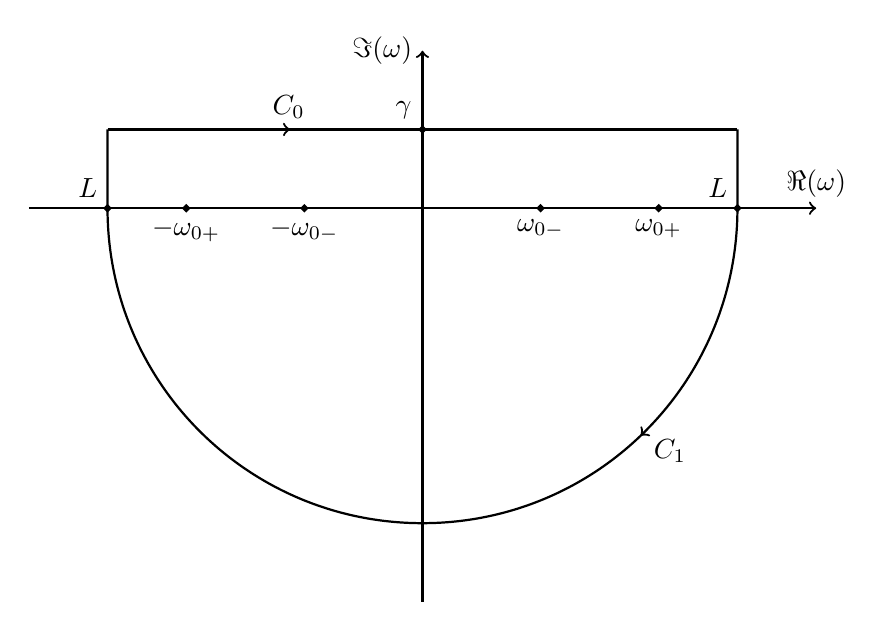
\begin{tikzpicture}[very thick,decoration={
			markings,
			mark=at position 0.29 with {\arrow{>}}}
		]
		\draw [->, thick] (-5,0) -- (5,0) node[above]{$\Re(\omega)$};
		\draw [->, thick] (0,-5) -- (0,2) node[left]{$\Im(\omega)$};
		
		\draw [postaction={decorate}, thick] (-4,1) -- (4,1);
		\draw [postaction={decorate}, thick] (4,1) to (4,0) node[above left]{$L$} to [out=-90,in=0] (0,-4) to [out=180,in=-90] (-4,0) node[above left]{$L$} to (-4,1);
		\node [above left] at (0,1) {$\gamma$};
		
		\draw[fill] (-4,0) circle [radius=0.025];
		\draw[fill] (4,0) circle [radius=0.025];
		\draw[fill] (0,1) circle [radius=0.025];
		
		\draw[fill] (3,0) circle [radius=0.025];
		\node [below] at (3,0) {$\omega_{0+}$};
		
		\draw[fill] (-3,0) circle [radius=0.025];
		\node [below] at (-3,0) {$-\omega_{0+}$};
		
		\draw[fill] (1.5,0) circle [radius=0.025];
		\node [below] at (1.5,0) {$\omega_{0-}$};
		
		\draw[fill] (-1.5,0) circle [radius=0.025];
		\node [below] at (-1.5,0) {$-\omega_{0-}$};
		
		\node [above] at (-1.7,1) {$C_0$};
		\node [below right] at (2.8,-2.8) {$C_1$};
		\end{tikzpicture} 
	}
	\caption{Bromwich contour for the complex integration of $\tilde{A}_{1,2}$.}
	\label{fig: brom cont incomp}
\end{figure}
Considering first the integral along $C_1$, the integrand in question behaves like $T_1(\omega)/kD(\omega) = \mathcal{O}(|\omega|^{-2})$, as $|\omega| \to \infty$. Therefore, the integral around the semi-circle vanishes, \textit{i.e.}
\begin{equation}
\lim_{L \to \infty} \int_{C_1} \frac{T_1(\omega)}{kD(\omega)} e^{-i\omega t} d\omega = 0.
\end{equation}

Next, the integral along contour $C$ is integrated in the clockwise direction it is therefore equal to $-2\pi i$ multiplied by the sum of the residues of the singularities at $\omega = \pm \omega_{0\pm}$. The residues are evaluated using L'Hopital's Rule (the requirements ensuring the validity of this rule are verified in Appendix~\ref{app: l'hopital}). For arbitrary choice of initial condition, $f(x,\omega)$, the residue at $\omega = \omega_{0+}$ is
\begin{align}
\mathrm{Res}&\left\{\frac{T_1(\omega)}{kD(\omega)}e^{-i\omega t}; \omega = \omega_{0+} \right\} = 
\lim_{\omega \to \omega_{0+}} \frac{(\omega - \omega_{0+})T_1(\omega)}{kD(\omega)} e^{-i\omega t} \notag \\ 
&= \lim_{\omega \to \omega_{0+}} \frac{1}{kD'(\omega)} [T_1(\omega) + (\omega - \omega_{0+})T'_1(\omega) - it(\omega - \omega_{0+})T_1(\omega)]e^{-i\omega t} \notag \\
&= \lim_{\omega \to \omega_{0+}} \frac{1}{kD'(\omega)} T_1\left[\omega \Psi_0 + i\frac{\partial \Psi_0}{\partial t}\right](\omega) e^{-i\omega t} \notag \\
&= \lim_{\omega \to \omega_{0+}} \frac{1}{kD'(\omega)} \left\{ \omega T_1[\Psi_0](\omega) + iT_1\left[\frac{\partial \Psi_0}{\partial t}\right](\omega) \right\} e^{-i\omega t} \notag \\
&= \left\{ \omega_{0+} \chi_{1+}[\Psi_0] + i\chi_{1+}\left[\frac{\partial \Psi_0}{\partial t}\right] \right\} e^{-i\omega_{0+} t},
\end{align}
where $\chi_{1+}[g] = T_1[g](\omega_{0+}) / kD'(\omega_{0+})$ is a functional mapping an arbitrary function $g$ to the real numbers. Similarly, the residues at $\omega = -\omega_{0+}$ and $\omega = \pm\omega_{0-}$ are
\begin{align}
\mathrm{Res}\left\{\frac{T_1(\omega)}{kD(\omega)}e^{-i\omega t}; \omega = -\omega_{0+} \right\} &= \left\{ \omega_{0+} \chi_{1+}[\Psi_0] - i\chi_{1+}\left[\frac{\partial \Psi_0}{\partial t}\right] \right\} e^{i\omega_{0+} t}, \\
\mathrm{Res}\left\{\frac{T_1(\omega)}{kD(\omega)}e^{-i\omega t}; \omega = \pm \omega_{0-} \right\} &= \left\{ \omega_{0-} \chi_{1-}[\Psi_0] \pm i\chi_{1-}\left[\frac{\partial \Psi_0}{\partial t}\right] \right\} e^{\mp i\omega_{0-} t},
\end{align}
respectively, where we define $\chi_{1-}[g] = T_1[g](\omega_{0-}) / kD'(\omega_{0-})$. To derive these residues, we have used the fact that $D'$ is an odd function of $\omega$, and $D$ and $T_1[g]$ are even functions of $\omega$, for any function $g$ that is constant with respect to $\omega$.

Compiling the above results, the solution of the first inverse Laplace Transform of Equation~\eqref{sol incomp} is
\begin{align}
\mathcal{L}^{-1}\left\{ \tilde{A}_1 \right\} &= \frac{1}{2\pi} \lim_{L \to \infty} \int_{C_0} \frac{T_1(\omega)}{kD(\omega)} e^{-i\omega t} d\omega \\
&= \frac{1}{2\pi} \lim_{L \to \infty} \int_{C} \frac{T_1(\omega)}{kD(\omega)} e^{-i\omega t} d\omega \notag \\
&= -i \sum \mathrm{Res}\left\{\frac{T_1(\omega)}{kD(\omega)}e^{-i\omega t}; \omega = \pm \omega_{0\pm} \right\} \notag \\
&= -i \left\{\omega_{0+}\chi_{1+}[\Psi_0] \left(e^{-i\omega_{0+} t} + e^{i\omega_{0+} t}\right) + i\chi_{1+}\left[ \frac{\partial \Psi_0}{\partial t} \right] \left(e^{-i\omega_{0+} t} - e^{i\omega_{0+} t}\right) \right. \notag \\
& \qquad\quad \left. + \omega_{0-}\chi_{1-}[\Psi_0] \left(e^{-i\omega_{0-} t} + e^{i\omega_{0-} t}\right) + i\chi_{1-}\left[ \frac{\partial \Psi_0}{\partial t} \right] \left(e^{-i\omega_{0-} t} - e^{i\omega_{0-} t}\right)\right\} \notag \\
&= -2 \left\{ i\omega_{0+}\chi_{1+}[\Psi_0] \cos(\omega_{0+} t) - \chi_{1+}\left[ \frac{\partial \Psi_0}{\partial t} \right] \sin(\omega_{0+} t) \right. \notag \\
& \qquad\quad \left. + i\omega_{0-}\chi_{1-}[\Psi_0] \cos(\omega_{0-} t) - \chi_{1-}\left[ \frac{\partial \Psi_0}{\partial t} \right] \sin(\omega_{0-} t) \right\}.
\end{align}


The second inverse Laplace transform in Equation~\eqref{sol incomp} is calculated as follows.
\begin{align}
\mathcal{L}^{-1}\left\{ \frac{\omega}{\e_1} \right\} &= \frac{1}{2\pi}\lim_{L \to \infty} \int_{i\gamma - L}^{i\gamma + L} \frac{\omega e^{-i\omega t}}{\e_1} ~d\omega \notag \\
&= \frac{1}{2\pi\rho_1}\lim_{L \to \infty} \int_{i\gamma - L}^{i\gamma + L} \frac{\omega e^{-i\omega t}}{(kv_{A1} + \omega)(kv_{A1} - \omega)} ~d\omega,
\end{align}
whose integrand has simple poles at $\omega = \pm k v_{A1}$. From Jordan's Lemma it follows that the integrand vanishes as $\omega \to \infty$, we can construct a Bromwich contour as shown in Figure~\ref{fig: brom cont incomp 2}. The residues of the integrand at the simple poles are
\begin{align}
\mathrm{Res}\left\{\frac{\omega e^{-i\omega t}}{k^2v_{A1}^2 - \omega^2}; \omega = \pm kv_{A1} \right\} &= 
\lim_{\omega \to \pm kv_{A1}} \frac{(\omega \mp kv_{A1}) \omega e^{-i\omega t}}{k^2v_{A1}^2 - \omega^2} \\ 
&= -\frac{1}{2}e^{\mp ikv_{A1} t}.
\end{align}
Therefore, the second inverse Laplace transform in Equation~\eqref{sol incomp} is
\begin{equation}
\mathcal{L}^{-1}\left\{ \frac{\omega}{\e_1} \right\} = -\frac{i}{\rho_1} \sum \mathrm{Res} \left\{ \frac{\omega e^{-i\omega t}}{k^2v_{A1}^2 - \omega^2}; \omega = \pm kv_{A1} \right\} = \frac{i}{\rho_1}\cos{kv_{A1}t}.
\end{equation}

The third and final inverse Laplace transform in Equation~\eqref{sol incomp} is calculated as follows.
\begin{align}
\mathcal{L}^{-1}\left\{ \frac{1}{\e_1} \right\} &= \frac{1}{2\pi}\lim_{L \to \infty} \int_{i\gamma - L}^{i\gamma + L} \frac{e^{-i\omega t}}{\e_1} ~d\omega, \notag \\
&= \frac{1}{2\pi\rho_1}\lim_{L \to \infty} \int_{i\gamma - L}^{i\gamma + L} \frac{e^{-i\omega t}}{(kv_{A1} + \omega)(kv_{A1} - \omega)} ~d\omega,
\end{align}
whose integrand has simple poles at $\omega = \pm k v_{A1}$. By noting that the integrand approaches zero as $\omega \to \infty$, we can construct a Bromwich contour as shown in Figure~\ref{fig: brom cont incomp 2}. The residues of the integrand at the simple poles are
\begin{align}
\mathrm{Res}\left\{\frac{e^{-i\omega t}}{k^2v_{A1}^2 - \omega^2}; \omega = \pm kv_{A1} \right\} &= 
\lim_{\omega \to \pm kv_{A1}} \frac{(\omega - kv_{A1}) e^{-i\omega t}}{k^2v_{A1}^2 - \omega^2} \notag \\ 
&= \mp \frac{1}{2kv_{A1}} e^{\mp ikv_{A1} t}.
\end{align}
Therefore, the final inverse Laplace transform in Equation~\eqref{sol incomp} is
\begin{align}
\mathcal{L}^{-1}\left\{ \frac{1}{\e_1} \right\} &= -\frac{i}{\rho_1} \sum \mathrm{Res} \left\{ \frac{e^{-i\omega t}}{k^2v_{A1}^2 - \omega^2}; \omega = \pm kv_{A1} \right\} \notag \\
&= \frac{1}{\rho_1kv_{A1}} \sin{kv_{A1}t}.
\end{align}

\begin{figure}
	\centering
	\scalebox{0.9}{
		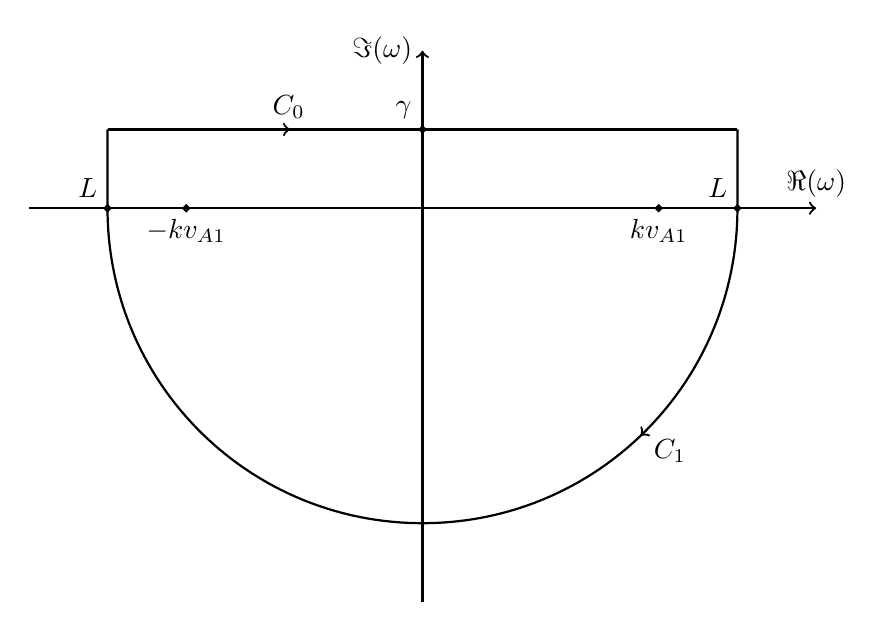
\begin{tikzpicture}[very thick,decoration={
			markings,
			mark=at position 0.29 with {\arrow{>}}}
		]
		\draw [->, thick] (-5,0) -- (5,0) node[above]{$\Re(\omega)$};
		\draw [->, thick] (0,-5) -- (0,2) node[left]{$\Im(\omega)$};
		
		\draw [postaction={decorate}, thick] (-4,1) -- (4,1);
		\draw [postaction={decorate}, thick] (4,1) to (4,0) node[above left]{$L$} to [out=-90,in=0] (0,-4) to [out=180,in=-90] (-4,0) node[above left]{$L$} to (-4,1);
		\node [above left] at (0,1) {$\gamma$};
		
		\draw[fill] (-4,0) circle [radius=0.025];
		\draw[fill] (4,0) circle [radius=0.025];
		\draw[fill] (0,1) circle [radius=0.025];
		
		\draw[fill] (3,0) circle [radius=0.025];
		\node [below] at (3,0) {$kv_{A1}$};
		
		\draw[fill] (-3,0) circle [radius=0.025];
		\node [below] at (-3,0) {$-kv_{A1}$};
		
		\node [above] at (-1.7,1) {$C_0$};
		\node [below right] at (2.8,-2.8) {$C_1$};
		\end{tikzpicture} 
	}
	\caption{Bromwich contour for the complex integration of the integrand of $J_1$.}
	\label{fig: brom cont incomp 2}
\end{figure}
Combining the above expressions for the inverse Laplace transforms, we find that the transverse velocity solution for $x<-x_0$ is
\begin{align}
v_x(x, t) = &-2 e^{k(x+x_0)} \left\{ i\omega_{0+}\chi_{1+}[\Psi_0] \cos(\omega_{0+} t) - \chi_{1+}\left[ \frac{\partial \Psi_0}{\partial t} \right] \sin(\omega_{0+} t) \right. \\
&\left. + i\omega_{0-}\chi_{1-}[\Psi_0] \cos(\omega_{0-} t) - \chi_{1-}\left[ \frac{\partial \Psi_0}{\partial t} \right] \sin(\omega_{0-} t) \right\} \\
&+ \frac{i}{\rho_1} \int_{-\infty}^{-x_0} G_1(x;s) \left[ \Psi(s, 0) \cos{kv_{A1}t} + \frac{\partial \Psi}{\partial t}(s, 0) \frac{\sin{kv_{A1}t}}{kv_{A_1}} \right]~ds.
\end{align}
Similarly, the transverse velocity for the region $x>x_0$ is
\begin{align}
v_x(x, t) = &-2 e^{k(x_0 - x)} \left\{ i\omega_{0+}\chi_{2+}[\Psi_0] \cos(\omega_{0+} t) - \chi_{2+}\left[ \frac{\partial \Psi_0}{\partial t} \right] \sin(\omega_{0+} t) \right. \notag \\
&\left. + i\omega_{0-}\chi_{2-}[\Psi_0] \cos(\omega_{0-} t) - \chi_{2-}\left[ \frac{\partial \Psi_0}{\partial t} \right] \sin(\omega_{0-} t) \right\} \notag \\
& + \frac{i}{\rho_2} \int_{x_0}^{\infty} G_2(x;s) \left[ \Psi(s, 0) \cos{kv_{A2}t} + \frac{\partial \Psi}{\partial t}(s, 0) \frac{\sin{kv_{A2}t}}{kv_{A_2}} \right]~ds.
\end{align}
Finally, for the region $|x|<x_0$, it is
\begin{align}
v_x(x, t) =& -\frac{2}{\sinh{2kx_0}} \left[ \left\{ i\omega_{0+}\chi_{1+}[\Psi_0] \cos(\omega_{0+} t) - \chi_{1+}\left[ \frac{\partial \Psi_0}{\partial t} \right] \sin(\omega_{0+} t) \right. \right. \notag \\
& \left. + i\omega_{0-}\chi_{1-}[\Psi_0] \cos(\omega_{0-} t) - \chi_{1-}\left[ \frac{\partial \Psi_0}{\partial t} \right] \sin(\omega_{0-} t) \right\} \sinh(k(x_0 - x)) \notag \\ 
& + \left\{ i\omega_{0+}\chi_{2+}[\Psi_0] \cos(\omega_{0+} t) - \chi_{2+}\left[ \frac{\partial \Psi_0}{\partial t} \right] \sin(\omega_{0+} t) \right. \notag \\
& \left. \left. + i\omega_{0-}\chi_{2-}[\Psi_0] \cos(\omega_{0-} t) - \chi_{2-}\left[ \frac{\partial \Psi_0}{\partial t} \right] \sin(\omega_{0-} t) \right\} \sinh(k(x_0 + x)) \right] \notag \\
& + \frac{i}{\rho_0} \int_{-x_0}^{x_0} G_0(x;s) \left[ \Psi(s, 0) \cos{kv_{A0}t} + \frac{\partial \Psi}{\partial t}(s, 0) \frac{\sin{kv_{A0}t}}{kv_{A0}} \right]~ds.
\end{align}


\subsubsection{Uniform initial vorticity}

Let $\Omega(x, 0) = \Omega_0$ be constant. Therefore, $\Psi_0 = k\rho_0\Omega_0$ and $\partial \Psi_0 / \partial t = 0$. To evaluate the solution, we evaluate each Green's function integral separately:
\begin{align}
\int_{-\infty}^{-x_0} G_1(x;s) \Psi_0 ~ds &= \Omega_0 \rho_1 \left[ \sinh(k(x+x_0)) \int_{-\infty}^{x} e^{k(s + x_0)} ~ds \right . \notag \\
&\qquad \qquad \left.+ e^{k(x+x_0)} \int_{x}^{-x_0} \sinh(k(s+x_0)) ~ds \right] \notag \\
&= \frac{\Omega_0 \rho_1}{k} \left[ e^{k(x+x_0)} - 1 \right].
\end{align}

\begin{align}
\int_{-x_0}^{x_0} G_0(x;s) \Psi_0 ~ds &= \frac{\Omega_0 \rho_0}{\sinh{2kx_0}} \left[ \sinh(k(x-x_0)) \int_{-x_0}^{x} \sinh(k(s+x_0)) ~ds \right. \notag \\
&\qquad \qquad \qquad \left. + \sinh(k(x+x_0)) \int_{x}^{x_0} \sinh(k(s-x_0)) ~ds \right], \notag \\
&= \frac{\Omega_0 \rho_0}{k} \left( \frac{\cosh{kx}}{\cosh{kx_0}} - 1 \right).
\end{align}

\begin{align}
\int_{x_0}^{\infty} G_2(x;s) \Psi_0 ~ds &= - \Omega_0 \rho_2 \left[ e^{-k(x-x_0)} \int_{x_0}^{x} \sinh(k(s-x_0)) ~ds \right. \notag \\
&\qquad \qquad \quad \left. + \sinh(k(x-x_0)) \int_{x}^{\infty} e^{-k(s-x_0)} ~ds \right], \notag \\
&= \frac{\Omega_0 \rho_2}{k} \left[ e^{-k(x-x_0)} - 1 \right].
\end{align}

\begin{align}
I_0^\pm &= \frac{\Omega_0\omega\rho_0k}{\sinh{2kx_0}} \int_{-x_0}^{x_0} \sinh(k(s \pm x_0)) ds, \\
&= \pm \frac{\Omega_0 \omega \rho_0}{\sinh{2kx_0}} (\cosh{2kx_0 - 1}).
\end{align}

\begin{align}
I_1 &= \Omega_0\omega\rho_1k \int_{-\infty}^{-x_0} e^{k(s + x_0)} ds, \\
&= \Omega_0 \omega \rho_1.
\end{align}

\begin{align}
I_2 &= \Omega_0\omega\rho_2k \int_{x_0}^{\infty} e^{k(x_0 - s)} ds, \\
&= \Omega_0 \omega \rho_2.
\end{align}
Using the above integrals, the transverse velocity through time for an initially constant vorticity is
\begin{equation}
v_x = -\frac{i}{k}\begin{cases}
2 e^{k(x+x_0)} A^*_1 + \Omega_0 \left\{1 - e^{k(x+x_0)}\right\} \cos{kv_{A1}t} \quad &\text{ for } x<-x_0, \\
\frac{2}{\sinh{2kx_0}} \left[ A^*_1 \sinh(k(x_0 - x)) + A^*_2 \sinh(k(x_0 + x)) \right] & \\
+ \Omega_0 \left( 1 - \frac{\cosh{kx}}{\cosh{kx_0}} \right)\cos{kv_{A0}t} \quad &\text{ for } x < |x_0|, \\
2 e^{k(x_0-x)} A^*_2 + \Omega_0 \left\{1 - e^{k(x_0-x)}\right\} \cos{kv_{A2}t} \quad &\text{ for } x>x_0, \\
\end{cases}
\label{sol slab}
\end{equation}
where
\begin{equation}
A^*_{1,2} = \omega_{0+} \frac{T_{1,2}[\psi_0](\omega_{0+})}{D'(\omega_{0+})} \cos(\omega_{0+} t) + \omega_{0-}\frac{T_{1,2}[\psi_0](\omega_{0-})}{D'(\omega_{0-})} \cos(\omega_{0-} t),
\end{equation}
and
\begin{align}
T_{1,2}[\Psi_0](\omega) = &-\Omega_0\{ (\rho_0 \tanh(kx_0) + \rho_{1,2}) (\e_0 \cosh(2kx_0) + \e_{2,1}\sinh(2kx_0)) \notag \\
&+ \e_0(\rho_0 \tanh(kx_0) + \rho_{2,1}) \}.
\end{align}

When $\rho_1 = \rho_2 = \rho_0$ and $x_0 = 0$, the solution given by Equation~\eqref{sol slab} reduces with that of a tangential interface, Equation~\eqref{sol int}.

\textcolor{red}{include figures of the solution}

The time-dependant evolution of a perturbation of an incompressible asymmetric magnetic slab are thus purely superposition of normal modes. There is no contribution from the continuous spectrum. There is instantaneous set-up of coherently oscillating collective modes. It is the introduction of compressibility that introduces a continuous spectrum, and therefore a leaky component to the oscillation. This is the subject of the following subsection.


\subsection{Compressible}

\textcolor{red}{Subsection intro - just a sentence or short para about what we might expect to come up in the compressible case.}

To tackle the more general compressible model, we must start with the more general version of Equation \eqref{gov reduced}, namely,
\begin{equation}
\tilde{v}_x - m^2 \tilde{v}_x = g(x, \omega),
\end{equation}
where
\begin{equation}
g(x, \omega) = \frac{1}{(c_0^2 + v_A^2)(\omega_T^2 - \omega^2)}\left[ (\omega_0^2 - \omega^2)\left(\dot{\hat{v}}_{x0} - i\omega \hat{v}_{x0}\right) + ikc_0^2\left( \dot{\hat{v}}_{z0}' - i\omega \hat{v}_{z0}'\right) \right].
\end{equation}
This equation corroborates with the general initial value problem considered by \cite{and_etal07}, although some algebra is required to transform between velocity and total pressure coordinates.

Considering a magnetic slab in a non-magnetic environment, we have
\begin{align}
m_0^2 &= \frac{(\omega_0^2 - \omega^2)(\omega_A^2 - \omega^2)}{(c_0^2 + v_A^2)(\omega_T^2 - \omega^2)}, \quad m_{1,2}^2 = \frac{\omega_{1,2}^2 - \omega^2}{c_{1,2}^2}, \\
g_{1,2}(x, \omega) &= \frac{1}{c_0^2\omega^2} \left[ (\omega_0^2 - \omega^2)\left(\dot{\hat{v}}_{x0} - i\omega \hat{v}_{x0}\right) + ikc_0^2\left( \dot{\hat{v}}_{z0}' - i\omega \hat{v}_{z0}'\right) \right].
\end{align}


\subsubsection{Solution in Laplace space}

For the solution inside the slab, $|x| < x_0$, $\hat{v}_x(x)$ satisfies
\begin{equation}
\left( \frac{\partial^2}{\partial x^2} - m_0^2 \right) \tilde{v}_x = g_0(\omega, x),
\end{equation}
under the boundary conditions $\tilde{v}_x(-x_0) = \tilde{A}_1$ and $\tilde{v}_x(-x_0) = \tilde{A}_2$. To solve this we construct the Green's function, $G_0(x;s)$ that satisfies
\begin{equation}
\frac{d^2G_0}{dx^2} - m_0^2 G_0 = \delta(x-s), \quad G_0(-x_0;s) = G_0(x_0;s) = 0,
\end{equation}
where $\delta$ denotes the Dirac delta function. The general solution of this equation is
\begin{equation}
G_0(x;s) = c_1\sinh(m_0(x - x_0)) + c_2\sinh(m_0(x + x_0)),
\end{equation}
where $c_1 = 0$ for $x < s$ and $c_2 = 0$ for $x > s$. Ensuring $G_0$ and $\partial G_0 / \partial x$ have jumps of 0 and 1 at $x = s$, respectively, determines $c_1$ and $c_2$ so that $G_0(x;s)$ is
\begin{equation}
G_0(x;s) = \frac{-1}{m_0\sinh(2m_0 x_0)}
\begin{cases}
\sinh(m_0(x_0 - s))\sinh(m_0(x_0 + x)), & \text{if } -x_0<x<s, \\
\sinh(m_0(x_0 - x))\sinh(m_0(x_0 + s)), & \text{if } s<x<x_0.
\end{cases}
\end{equation}
Then the solution of Equation~\eqref{P eq inside} is
\begin{align}
\tilde{v}_x(x) = &\frac{1}{m_0\sinh{2m_0 x_0}} \left[ \tilde{A}_1\sinh(m_0(x_0 - x)) + \tilde{A}_2\sinh(m_0(x_0 + x)) \right] \notag \\
&+ \int_{-x_0}^{x_0} G_0(x;s) g_0(\omega, s) ~ds.
\label{V sol 0}
\end{align}
This is the sum of the Green's function term and a two terms that are independent solutions to the homogeneous version of Equation~\eqref{P eq inside} that ensure that the inhomogeneous boundary conditions are satisfied.

For the solution outside and to the left of the slab, $x < -x_0$, $\tilde{v}_x(x)$ satisfies
\begin{equation}
\left(\frac{d^2}{dx^2} - m_1^2 \right) \tilde{v}_x = g_1(\omega, x),
\end{equation}
and the boundary conditions $\tilde{v}_x(-\infty) = 0$, $\tilde{v}_x(-x_0) = \tilde{A}_1$. By following a Green's function method, the solution of this Sturm-Liouville system is
\begin{equation}
\tilde{v}_x(x) = \tilde{A}_1e^{m_1(x_0+x)} + \int_{-\infty}^{-x_0} G_1(x; s) g_1(\omega, s) ds,
\label{V sol 1}
\end{equation}
where $m_1 > 0$ and the Green's function, $G_1$, is defined by
\begin{equation}
G_1(x; s) = \frac{1}{m_1}
\begin{cases}
e^{m_1(x_0 + x)}\sinh(m_1(x_0 + s)), & \text{if } x < s, \\
e^{m_1(x_0 + s)}\sinh(m_1(x_0 + x)), & \text{if } s < x < -x_0.
\end{cases}
\end{equation}

Similarly, the solution outside and to the right of the slab, $x > x_0$, is
\begin{equation}
\tilde{v}_x(x) = \tilde{A}_2e^{m_2(x_0-x)} + \int_{x_0}^{\infty} G_2(x; s) g_2(\omega, s) ~ds,
\label{P sol 2}
\end{equation}
where $m_2 > 0$ and the Green's function, $G_2$, is defined by
\begin{equation}
G_2(x; s) = \frac{1}{m_2}
\begin{cases}
e^{m_2(x_0 - s)}\sinh(m_2(x_0 - x)), & \text{if } x_0 < x < s, \\
e^{m_2(x_0 - x)}\sinh(m_2(x_0 - s)), & \text{if } s < x.
\end{cases}
\end{equation}

Putting all of this together, the Laplace transform of the transverse velocity is
\begin{equation}
\tilde{v}_x(x) = 
\begin{cases}
\tilde{A}_1e^{m_1(x_0 + x)} + \int_{-\infty}^{-x_0} G_1(x; s) g_1(\omega, s) ~ds, & \text{if } -\infty < x < -x_0, \\

\frac{1}{\sinh{2m_0x_0}} \left[ \tilde{A}_1\sinh(m_0(x_0 - x)) + \tilde{A}_2\sinh(m_0(x_0 + x)) \right]  \\
+ \int_{-x_0}^{x_0} G_0(x; s) g_0(\omega, s) ~ds, & \text{if } |x| < x_0, \\

\tilde{A}_2e^{m_2(x_0 - x)} + \int_{x_0}^{\infty} G_2(x; s) g_2(\omega, s) ~ds, & \text{if } x_0 < x < \infty.
\end{cases}
\label{V sol}
\end{equation}


\subsubsection{Matching solutions}

For physically relevant solutions, we require that the transverse velocity) and the total pressure be continuous across the interfaces at $x = \pm x_0$.

Continuity in transverse velocity, $\tilde{v}_x$, is satisfied automatically by considering the solutions inside and outside the slab given by Equations~\eqref{V sol 0},~\eqref{V sol 1}, and~\eqref{V sol 2}, respectively, and our definition of $\tilde{A}_1 = \tilde{v}_x(-x_0)$ and $\tilde{A}_2 = \tilde{v}_x(x_0)$.

Continuity in total pressure can be dealt with as follows. The perturbation in total pressure is related to the velocity gradient by\footnote{Found by combining that induction equation with the momentum equation, see, for example, the bottom row of Equation~(2) by \cite{and_etal07}.}
\begin{equation}
\frac{\partial p_T}{\partial t} = -\rho\left[ \left(c_0^2 + v_A^2\right) \frac{\partial v_x}{\partial x} + c_0^2\frac{\partial v_z}{\partial z} \right].
\end{equation}
Looking for solutions proportional to $\exp{ikz}$ and taking Laplace transforms in time leads to
\begin{equation}
\tilde{p}_T = -\frac{i\rho}{\omega} \frac{(c_0^2 + v_A^2)(\omega_T^2 - \omega^2)}{(\omega_0^2 - \omega^2)} \tilde{v}_x' + \frac{i}{\omega} \hat{p}_{T0} + \frac{\rho \omega^2}{k\omega(\omega_0^2 - \omega^2)} \left(\dot{\hat{v}}_{z0} - i\omega\hat{v}_{z0}\right).
\end{equation}
Therefore, if we make the simplification\footnote{This simplification is not as strict as it might first seem. For example, any pressure perturbation-free transverse kick, such as you might expect from a nearby flare, would do.} to the prescribed initial conditions such that
\begin{equation}
\hat{p}_{T0} - \frac{\rho \omega_0^2}{k(\omega_0^2 - \omega^2)} \left(i\hat{v}_{z0} + \omega\dot{\hat{v}}_{z0}\right) = 0,
\end{equation}
then the continuity in total pressure boundary condition is equivalent to
\begin{equation}
\left[ \left[ \frac{\Lambda}{m} \frac{\partial \tilde{v}_x}{\partial x} \right] \right]_{x=\pm x_0} = 0,
\end{equation}
where double brackets indicate a jump in the quantity,
\begin{equation}
[[f]]_{x=x_0} = \lim_{\epsilon \to 0} [f(x_0 + \epsilon) - f(x_0 - \epsilon)].
\end{equation}
\textcolor{red}{check we havent redefined lambda.}

Substituting the solutions given by Equations~\eqref{P sol 0}, \eqref{P sol 1}, and~\eqref{P sol 2} into these boundary conditions gives
\begin{equation}
\tilde{A}_1(\omega) = \frac{T_1(\omega)}{D(\omega)}, \quad \tilde{A}_2(\omega) = \frac{T_2(\omega)}{D(\omega)},
\end{equation}
where
\begin{align}
T_1(\omega) = T_1[f](\omega) = & -(\Lambda_0\cosh{2m_0 x_0} + \Lambda_2\sinh{2m_0 x_0})(\Lambda_0 I_0^- + \Lambda_1 I_1) \notag \\
& - \Lambda_0(\Lambda_0 I_0^+ + \Lambda_2 I_2), \\
T_2(\omega) = T_2[f](\omega) = & - (\Lambda_0\cosh{2m_0 x_0} + \Lambda_1\sinh{2m_0 x_0})(\Lambda_0 I_0^+ + \Lambda_2 I_2) \notag \\
& -\Lambda_0(\Lambda_0 I_0^- + \Lambda_1 I_1), \\
D(\omega) = & \Lambda_0(\Lambda_1 + \Lambda_2)\cosh(2m_0x_0) + (\Lambda_0^2 + \Lambda_1\Lambda_2)\sinh(2m_0x_0),
\label{D}
\end{align}
where $\Lambda_j = \rho_j (\omega^2 - \omega_{Aj}^2) /  m_j$, for $j = 0, 1, 2$, and
\begin{align}
I_0^\pm &= I_0^\pm[f] = \frac{1}{m_0} \int_{-x_0}^{x_0} \frac{\sinh(m_0(x_0 \pm s))}{\sinh(2m_0x_0)} f(\omega, s) ~ds, \\
I_1 &= I_1[f] = \frac{1}{m_1} \int_{-\infty}^{-x_0} e^{m_1(s + x_0)} f(\omega, s) ~ds, \\
I_2 &= I_2[f] = \frac{1}{m_2} \int_{x_0}^\infty e^{m_2(x_0 - s)} f(\omega, s) ~ds.
\end{align}


\subsubsection{Solution in time}

To recover the transverse velocity, $v_x(x, t)$, we employ the inverse Laplace transform (non-standard, discussed in Appendix~\ref{app: laplace trans}), such that
\begin{equation}
\hat{v}_x(x,t) = \mathcal{L}^{-1}\{\tilde{v}_x(x)\} = \frac{1}{2\pi} \lim_{L \to \infty} \int_{i\gamma - L}^{i\gamma + L} \tilde{v}_x(x) e^{-i\omega t} d\omega,
\label{laplace transform}
\end{equation}
where $\gamma$ is a real number such that all the singularities of the integrand are below the contour of integration to ensure that all singularities contribute to the integral. The integral is evaluated along an infinite horizontal line in the upper half of the complex plane and is dependent on the singularities (with respect to $\omega$) of $\tilde{v}_x$, whose residues determine the value of the contour integral. Focusing firstly on the region $x < -x_0$, the solution is
\begin{align}
\hat{v}_x(x, t) &= \mathcal{L}^{-1} \left\{ \tilde{A}_1 e^{m_1(x + x_0)} + \int_{-\infty}^{-x_0} G_1(x; s)f_1(\omega, s)ds \right\}, \\
&= \mathcal{L}^{-1} \left\{ \tilde{A}_1 e^{m_1(x + x_0)} \right\} + \mathcal{L}^{-1} \left\{ \int_{-\infty}^{-x_0} G_1(x; s)f_1(\omega, s)ds \right\}.
\end{align}
The inverse Laplace transform in this solution are evaluated in the following subsection. 

\textcolor{red}{ From R and R 06: Recall that the Laplace transform of a solution of any initial value problem is only valid when the imaginary part $\Im(\omega)$ of the complex frequency $\omega$ is larger than the maximum growth rate of perturbations. For a well-posed problem the perturbation growth rate is always bounded. In the particular case of a straight, untwisted, magnetic tube of interest here there is no reason to expect the existence of growing perturbations, since there are no instabilities, so that the maximum growth rate is zero; consequently, the Laplace transform is valid for $\Im(\omega) > 0$. After obtaining the Laplace transformed solution, we construct its analytic continuation into the lower part of the $\omega$-plane, $\Im(\omega) < 0$, allowing us to calculate the asymptotic behaviour of the solution for large times, $t \to \infty$.}

\color{red}
\subsubsection{Asymptotic solution for large time}

To study the asymptotic behaviours of the total pressure perturbation, we start with the asymptotic behaviours of $A_1(t) = v_x(-x_0, t)$ and $A_2(t) = v_x(x_0, t)$. These variables can be determined, using the inverse Laplace transform (non-standard, discussed in Appendix~\ref{app: laplace trans}), to be
\begin{equation}
A_1(t) = \frac{1}{2\pi} \lim_{L \to \infty} \int_{i\gamma - L}^{i\gamma + L} \frac{T_1(\omega)}{D(\omega)} e^{-i\omega t} d\omega, \quad A_2(t) = \frac{1}{2\pi} \lim_{L \to \infty} \int_{i\gamma - L}^{i\gamma + L} \frac{T_2(\omega)}{D(\omega)} e^{-i\omega t} d\omega,
\label{A inv laplace}
\end{equation}
where $\gamma$ is a real number such that all the singularities of the integrands are below the contour of integration. The integrals are evaluated along an infinite horizontal line in the upper half of the complex plane.

Since the problem of finding the solution is now reduced to solving a complex integral, it is dependent on the singularities (with respect to $\omega$) of $T_1$, $T_2$, and $D$ (so that we can construct a Bromwich contour such that it is confined to a single-valued branch) and the zeros of $D$ (whose residues determine the value of the contour integral).

To determine the singularities of these functions, we determine the singularities of the constituent functions, as follows.
\begin{itemize}
	\item The functions $\Lambda_j^2$ are rational functions of $\omega$ with simple poles at $\omega = \pm \omega_{0j}$, for $j = 0, 1, 2$.
	
	\item $\Lambda_j$, for $j = 0, 1, 2$, involve radicals and have (algebraic) branch points at $\omega = \pm \omega_{Aj}$, $\pm \omega_{0j}$, and $\pm \omega_{Tj}$, respectively.\footnote{More precisely, $\omega = \pm \omega_{Aj}$, $\pm \omega_{0j}$, and $\pm \omega_{Tj}$ are the ramification points corresponding to the branch points $\Lambda_j(\omega)$, each with ramification index 2. However, the language used in the main text is common shorthand that is considered synonymous.}
	
	\item The functions $\cosh(z)$ and $\sinh(z)$ are entire functions of $z$ with only even and odd terms in their respective series expansions. Therefore, $\cosh(z)$ and $z\sinh(z)$ are entire functions of $z^2$. Hence, $\cosh(2m_0x_0)$ and $\Lambda_0\sinh{2m_0x_0}$ have only simple poles at $\omega = \omega_{T0}$.
	
	\item The integrands of $I_0^\pm$ are integrated with respect to $s$. Therefore, the singularities of $I_{1,2}$ are precisely the singularities of the integrands. The function $g(z) = \sinh(az) / \sinh(bz)$, for constants $a$ and $b \neq 0$ are entire functions of $z$, containing only even powers (once $g$ has been redefined as to remove the removable singularity at $z = 0$). Therefore, for another complex function $h$, the singularities of the composition $g \cdot h$ are precisely the singularities of the function $h(z^2)$. Hence, by letting $h(\omega) = m_0$, $a = s \pm x_0$, and $b = 2x_0$, it follows that $\sinh(m_0(s - x_0)) / \sinh(2m_0x_0)$ has simple poles at $\omega = \pm \omega_{T0}$.
	
	\item To determine the singularities of $I_{1,2}$, we need consider the singularities of the integrands. The functions $e^{a\sqrt{z}}$ and $e^{\frac{a}{\sqrt{z}}}$, for constant $a \neq 0$ have branch points at $z = 0$ that are algebraic (of ramification index 2) and transcendental, respectively. Therefore, by setting $a = x_0 \pm s$, it follows that the functions $e^{m_j(x_0 \pm s)}$, and therefore $I_j$, have algebraic branch points at $\omega = \pm \omega_{Aj}$ and $\pm \omega_{0j}$ and transcendental branch points at $\pm \omega_{Tj}$.
\end{itemize}
By the algebra of branch points, the set of branch points of a sum of functions is the union of the branch points of the constituent functions. Therefore, the branch points of both $T_1$ and $T_2$ are $\omega = \pm \omega_{A0,1,2}$ (algebraic), $\pm \omega_{00,1,2}$ (algebraic), $\pm \omega_{T0}$ (algebraic), and $\pm \omega_{T1,2}$ (transcendental). The dispersion function $D$ has branch points at $\omega = \pm \omega_{A0,1,2}$, $\pm \omega_{00,1,2}$, and $\pm \omega_{T0,1,2}$, all of which are algebraic.

\textcolor{red}{TO DO: Redo the above to show that we have algebraic branch points at all of the $\omega_{A,0,T}$ corresponding to the Alfven, slow and fast continua, corresponding to leaky modes. So we have 18 branch points. How should be choose the branch cuts? We need to ensure we are confined to a single Riemann sheet i.e. single valued. See e.g. Fig 6 in Sedlacek 1970.}

\textit{The above analysis determines that the singularities of each function $T_1(\omega)$, $T_2(\omega)$, and $D(\omega)$ are precisely the algebraic branch points at $\omega = \pm kv_{A1}$ and $\omega = \pm kv_{A2}$.}

The apparent singularity at the tube frequency in the inhomogeneous part of the governing equation, Equation~\eqref{}, is neutralised by multiplication by the Green's function \citep{and_etal07}. \textcolor{red}{SHOW THIS EXPLICITLY?}

\subsection{Asymptotic solution - non-magnetic external plasma}
If the external plasma is non-magnetic, \textit{i.e.} $v_{A1} = v_{A2} = 0$, then the integral has (algebraic) branch points at $\omega = \pm \omega_{A0}$, $\pm \omega_{00,1,2}$, and $\pm \omega_{T0}$, where, without loss of generality, we let $\omega_1 < \omega_2$. The contour, $C = C_1 + C_2 + C_3 + C_4 + C_5$ for the inverse Laplace transform can be modified as shown in Figure~\ref{fig: brom contour}. To ensure that the contour remains on a single Riemann surface, it is modified around the branch cuts so as to encircle the poles. The closed contour $C$ is a sum of the following sub-contours:
\begin{itemize}
	\item $C_0$: the horizontal line with imaginary part $\gamma$.
	\item $C_1$: the horizontal line from $L + \delta i$ to $\omega_0 + \delta i$, round the semicircle of radius $\delta$ and back along the horizontal line from $\omega_0 - \delta i$ to $L - \delta i$.
	\item $C_2$: the vertical lines from $\pm L + \gamma i$ to $\pm L + \delta i$ and the arcs of the large semicircle centred at the origin with radius $\Delta$.
	\item $C_3$: the vertical line up to, around, and back down from $\omega_T$.
	\item $C_4$: the vertical line up to, around, and back down from $-\omega_T$.
	\item $C_5$: the horizontal line from $-L - \delta i$ to $-\omega_0 - \delta i$, round the semicircle of radius $\delta$ and back along the horizontal line from $-\omega_0 + \delta i$ to $-L + \delta i$.
\end{itemize}
We use the integral along $C$ as $\delta \to 0$ and $L \to \infty$ to determine the inverse Laplace transform from Equation~\eqref{A inv laplace}. In the limit of $L \to \infty$, the integral along $C_0$ is identical to the desired integral in Equation~\eqref{A inv laplace}. The integrals along each of the sub-contours $C_1 - C_5$ are calculated in the following subsections.

\begin{figure}
	\centering
	\scalebox{0.9}{
		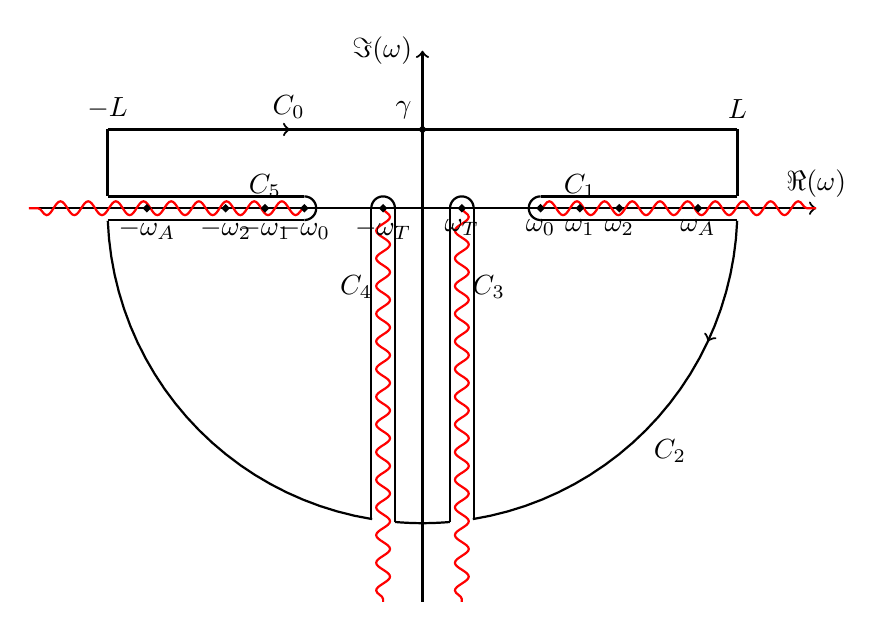
\begin{tikzpicture}[very thick, decoration={
			markings,
			mark=at position 0.29 with {\arrow{>}}}
		]
		
		\tikzset{
			branchcut/.style={decorate, decoration={snake}, draw=red}, 
		}
		
		\draw [->, thick] (-5,0) -- (5,0) node[above]{$\Re(\omega)$};
		\draw [->, thick] (0,-5) -- (0,2) node[left]{$\Im(\omega)$};
		
		\draw [postaction={decorate}, thick] (-4,1) -- (4,1);
		\draw [thick] (-4,1) -- (-4,0.15);
		\draw [thick] (4,1) -- (4,0.15);
		\draw [thick] (-4,0.15) -- (-1.5,0.15);
		\draw [thick] (4,0.15) -- (1.5,0.15);
		\draw [thick] (-4,-0.15) -- (-1.5,-0.15);
		\draw [thick] (4,-0.15) -- (1.5,-0.15);
		
		\draw [branchcut, thick] (0.5, 0) -- (0.5, -5);
		\draw [branchcut, thick] (-0.5, 0) -- (-0.5, -5);
		\draw [branchcut, thick] (1.5, 0) -- (5, 0);
		\draw [branchcut, thick] (-1.5, 0) -- (-5, 0);
		
		\draw [thick,domain=90:-90] plot ({0.15*cos(\x) - 1.5}, {0.15*sin(\x)});
		\draw [thick,domain=90:270] plot ({0.15*cos(\x) + 1.5}, {0.15*sin(\x)});
		
		\draw [postaction={decorate}, thick,domain=-2.3:-80.8] plot ({4*cos(\x)}, {4*sin(\x)});
		\draw [thick,domain=-85:-95] plot ({4*cos(\x)}, {4*sin(\x)});
		\draw [thick,domain=182.3:260.8] plot ({4*cos(\x)}, {4*sin(\x)});
		
		\draw [thick] (-0.35,0) -- (-0.35,-3.99);
		\draw [thick] (0.35,0) -- (0.35,-3.99);
		
		\draw [thick] (-0.65,0) -- (-0.65,-3.94);
		\draw [thick] (0.65,0) -- (0.65,-3.94);
		
		\draw [thick,domain=180:0] plot ({0.15*cos(\x) - 0.5}, {0.15*sin(\x)});
		\draw [thick,domain=180:0] plot ({0.15*cos(\x) + 0.5}, {0.15*sin(\x)});
		
		\node [above left] at (0,1) {$\gamma$};
		
		\draw[fill] (0,1) circle [radius=0.025];
		
		\draw[fill] (3.5,0) circle [radius=0.025];
		\node [below] at (3.5,0) {$\omega_{A}$};
		
		\draw[fill] (-3.5,0) circle [radius=0.025];
		\node [below] at (-3.5,0) {$-\omega_{A}$};
		
		\draw[fill] (2.5,0) circle [radius=0.025];
		\node [below] at (2.5,0) {$\omega_{2}$};
		
		\draw[fill] (-2.5,0) circle [radius=0.025];
		\node [below] at (-2.5,0) {$-\omega_{2}$};
		
		\draw[fill] (2,0) circle [radius=0.025];
		\node [below] at (2,0) {$\omega_{1}$};
		
		\draw[fill] (-2,0) circle [radius=0.025];
		\node [below] at (-2,0) {$-\omega_{1}$};
		
		\draw[fill] (1.5,0) circle [radius=0.025];
		\node [below] at (1.5,0) {$\omega_{0}$};
		
		\draw[fill] (-1.5,0) circle [radius=0.025];
		\node [below] at (-1.5,0) {$-\omega_{0}$};
		
		\draw[fill] (0.5,0) circle [radius=0.025];
		\node [below] at (0.5,0) {$\omega_{T}$};
		
		\draw[fill] (-0.5,0) circle [radius=0.025];
		\node [below] at (-0.5,0) {$-\omega_{T}$};
		
		\node [above] at (-1.7,1) {$C_0$};
		\node [above] at (2,0) {$C_1$};
		\node [below right] at (2.8,-2.8) {$C_2$};
		
		\node [right] at (0.5,-1) {$C_3$};
		\node [left] at (-0.5,-1) {$C_4$};
		\node [above] at (-2,0) {$C_5$};
		
		\node [above] at (4,1) {$L$};
		\node [above] at (-4,1) {$-L$};
		\end{tikzpicture} 
	}
	\caption{The Bromwich contour, $C = C_1 + C_2 + C_3 + C_4 + C_5$, for the complex integration of $\tilde{A}_{1,2}$ in the inverse Laplace transform in Equation~\eqref{A inv laplace}. The radius of the large semicircle is $L$ and the radius of the small semicircles around the points $\pm \omega_0$ and $\pm \omega_T$ is $\delta$.}
	\label{fig: brom contour}
\end{figure}


\subsubsection{Integral along $C_1$ and $C_5$}
In the limit as $\delta \to 0$, the integral along the semicircular part of $C_1$ approaches 0 because the integrand is analytic in this limit and the length of the contour approaches zero.

As $L \to \infty$ the integrals along $C_1$ become
\begin{align}
I_{C_1} &= \int_{C_1} \frac{T_{1,2}}{D} e^{-i\omega t} d\omega \\
&= \int_{\infty}^{\omega_0} \frac{T_{1,2}^+}{D^+} e^{-i\omega t} d\omega + \int_{\omega_0}^{\infty} \frac{T_{1,2}^-}{D^-} e^{-i\omega t} d\omega \\
&= \int_{\omega_0}^{\infty} \left( \frac{T_{1,2}^-}{D^-} - \frac{T_{1,2}^+}{D^+} \right) e^{-i\omega t} d\omega,
\end{align}
where superscripts $+$ and $-$ indicate the value of the function above and below the horizontal branch cut $[\omega_0, \infty)$, respectively.

For values of $\omega$ between the branch points at $\omega_0$, $\omega_1$, $\omega_2$, and $\omega_A$, the integrand is analytic (except at the endpoints), therefore we can use integration by parts in these sub-intervals. For example, the integral over the sub-interval $(\omega_0, \omega_1)$ is
\begin{align}
I_{(\omega_0, \omega_1)} &= \int_{\omega_0}^{\omega_1} \left( \frac{T_{1,2}^-}{D^-} - \frac{T_{1,2}^+}{D^+} \right) e^{-i\omega t} d\omega \\
&= \frac{i}{t} \left\{ \left[ \left( \frac{T_{1,2}^-}{D^-} - \frac{T_{1,2}^+}{D^+} \right) e^{-i\omega t}\right]_{\omega_0}^{\omega_1} - \int_{\omega_0}^{\omega_1} \frac{d}{d\omega} \left( \frac{T_{1,2}^-}{D^-} - \frac{T_{1,2}^+}{D^+} \right) e^{-i\omega t} d\omega \right\}.
\end{align}
Given that $T_{1,2}^+(\omega_0)/D^\pm(\omega_0) = T_{1,2}^-(\omega_0)/D^\pm(\omega_0)$, the slowest decaying term is the first term on the right hand side evaluated at $\omega_1$, which decays like $\mathcal{O}(t^{-1})$ as $t \to \infty$. Repeating this for the other three intervals over which the integrand is analytic, and using the fact that $T_{1,2}^\pm(\omega)/D^\pm(\omega) \to 0$ as $|\omega| \to \infty$, we find that the slowest decaying terms decay like $\mathcal{O}(t^{-1})$ as $t \to \infty$. Therefore $I_{C_1} = \mathcal{O}(t^{-1})$ (and similarly $I_{C_5} = \mathcal{O}(t^{-1})$) as $t \to \infty$.


\subsubsection{Integral along \texorpdfstring{$C_2$}{C2}}
As $L \to \infty$, points that occupy the curve $C_2$ will behave like $|\omega| \to \infty$. When $|\omega| \to \infty$, $T_{1,2} = \mathcal{O}(|\omega|)$ and $D = \mathcal{O}(|\omega|^2)$, therefore the integrands behave like $T_{1,2}/D = \mathcal{O}(1/|\omega|)$. Therefore the integral around $C_2$ approaches $0$ as $L \to \infty$.


\subsubsection{Integral along $C_3$ and $C_4$}
In the limit as $\delta \to 0$, the integral along the semicircular part of $C_3$ approaches 0 because the integrand is analytic in this limit and the length of the contour approaches zero. As $L \to \infty$ and $\delta \to 0$, the integrals along $C_3$ become
\begin{align}
I_{C_3} &= \int_{C_3} \frac{T_{1,2}}{D} e^{-i\omega t} d\omega \\
&= \int_{\omega_T}^{\omega_T - \infty i} \left( \frac{T_{1,2}^-}{D^-} - \frac{T_{1,2}^+}{D^+} \right) e^{-i\omega t} d\omega,
\end{align}
where superscripts $+$ and $-$ indicate the value of the function to the right and left of the vertical branch cut $\omega_T + [0,\infty)i$, respectively. The integrand is analytic in the integration interval (except at the endpoints), so by integration by parts
\begin{equation}
I_{C_3} = \frac{i}{t} \left\{ \left[ \left( \frac{T_{1,2}^-}{D^-} - \frac{T_{1,2}^+}{D^+} \right) e^{-i\omega t}\right]_{\omega_T}^{\omega_T -\infty i} - \int_{\omega_T}^{\omega_T - \infty i} \frac{d}{d\omega} \left( \frac{T_{1,2}^-}{D^-} - \frac{T_{1,2}^+}{D^+} \right) e^{-i\omega t} d\omega \right\}.
\end{equation}
the first term is zero because $T_{1,2}^\pm(\omega)/D^\pm(\omega) \to 0$ as $|\omega| \to \infty$ and $T_{1,2}^+(\omega_T)/D^\pm(\omega_T) = T_{1,2}^-(\omega_T)/D^\pm(\omega_T)$. Therefore, using integration by parts for a second time,
\begin{align}
I_{C_3} &= -\frac{i}{t} \int_{\omega_T}^{\omega_T - \infty i} \frac{d}{d\omega} \left( \frac{T_{1,2}^-}{D^-} - \frac{T_{1,2}^+}{D^+} \right) e^{-i\omega t} d\omega \\
&= \frac{1}{t^2} \left\{ \left[ \frac{d}{d\omega} \left( \frac{T_{1,2}^-}{D^-} - \frac{T_{1,2}^+}{D^+} \right) e^{-i\omega t}\right]_{\omega_T}^{\omega_T -\infty i} - \int_{\omega_T}^{\omega_T - \infty i} \frac{d^2}{d\omega^2} \left( \frac{T_{1,2}^-}{D^-} - \frac{T_{1,2}^+}{D^+} \right) e^{-i\omega t} d\omega \right\} \\
&= \mathcal{O}(t^{-2}) \text{ as } t \to \infty.
\end{align}
Similarly, $I_{C_5} = \mathcal{O}(t^{-2})$ as $t \to \infty$.


\subsubsection{Poles (AKA eigenfrequencies)}
Let $v_A > c_i$ for $i = 0, 1, 2$, then there can exist, in general:
\begin{enumerate}
	\item 2 slow surface modes,
	\item an infinite number of slow body modes,
	\item 2 fast surface modes.
\end{enumerate}
1 and 2 exist for all values of $kx_0$. 3 exist only for $kx_0$ values greater than a cut-off value. Analytical expressions for the behaviour of the eigenmodes do not exist in general. It is at this point that we are forced to make two simplifications to the model:
\begin{itemize}
	\item The thin-slab approximation, so that $kx_0 \ll 1$
	\item The approximate symmetry simplification, so that $\rho_1 \approx \rho_2$.
\end{itemize}
The eigenmodes of an asymmetric magnetic slab under these simplifications are given by the following expressions:
\begin{itemize}
	\item Slow quasi-sausage surface modes:
	\begin{equation}
	\omega^2=k^2c_\textrm{T}^2\left[1-\frac{2(kx_0)(c_0^2-c_\textrm{T}^2)}{(c_0^2+v_\textrm{A}^2)\left(\frac{\rho_0}{\rho_1}\frac{(c_1^2-c_\textrm{T}^2)^{1/2}}{c_1}+\frac{\rho_0}{\rho_2}\frac{(c_2^2-c_\textrm{T}^2)^{1/2}}{c_2}\right)}\right],
	\label{thinslab slow saus surf}
	\end{equation}
	which is less than $k^2c_\textrm{T}^2$ and exists only when $c_1>c_\textrm{T}$ and $c_2>c_\textrm{T}$.
	\item If $c_1=c_2=c_\textrm{e}$ (and therefore $\rho_1=\rho_2=\rho_\textrm{e}$), then there exists a fast sausage surface mode:
	\begin{equation}
	\omega^2=k^2c_\textrm{e}^2\left(1-\left[\frac{\rho_\textrm{e}}{\rho_0}\frac{c_\textrm{e}^2(c_0^2-c_\textrm{e}^2)(kx_0)}{(c_0^2+v_\textrm{A}^2)(c_\textrm{T}^2-c_\textrm{e}^2)}\right]^2\right)
	\label{thinslab fast saus surf}
	\end{equation}
	in the thin slab limit.
	\item Slow quasi-kink surface mode:
	\begin{equation}
	\omega^2=\frac{k^2x_0v_\textrm{A}^2\left(\frac{\rho_0}{\rho_1}m_1+\frac{\rho_0}{\rho_2}m_2\right)}{\left(\frac{\rho_0}{\rho_1}m_1x_0+\frac{\rho_0}{\rho_2}m_2x_0\right)+2}\approx{}\frac{1}{2}k^2v_\textrm{A}^2\left(\frac{\rho_0}{\rho_1}+\frac{\rho_0}{\rho_2}\right)kx_0.
	\label{thinslab slow kink surf}
	\end{equation}
	\item Quasi-sausage body solutions:
	\begin{equation}
	\omega^2=k^2c_\textrm{T}^2\left(1+\frac{c_\textrm{T}^4(kx_0)^2}{c_0^2v_\textrm{A}^2\pi^2j^2}\right), \quad j=1,2,\ldots. \label{thinslab saus body}
	\end{equation}
	\item Quasi-kink body solutions:
	\begin{equation}
	\omega^2=k^2c_\textrm{T}^2\left(1+\frac{c_\textrm{T}^4(kx_0)^2}{c_0^2v_\textrm{A}^2\pi^2(j-\frac{1}{2})^2}\right), \quad j=1,2,\ldots. \label{thinslab kink body}
	\end{equation}
\end{itemize}

Solution of the inverse Laplace transform is the sum of the residues at these points.

As shown in Appendix~\ref{app: approx sym DR}, under the approximate symmetry simplification, the dispersion function, $D(\omega)$, becomes
\begin{equation}
D(\omega) = \frac{\sinh{2m_0x_0}}{4\Lambda_1\Lambda_2} D_k(\omega) D_s(\omega),
\end{equation}
where
\begin{align}
D_k(\omega) &= \Lambda_0 (\Lambda_1 + \Lambda_2) + 2\Lambda_1\Lambda_2\coth(m_0x_0), \\
D_s(\omega) &= \Lambda_0(\Lambda_1 + \Lambda_2) + 2\Lambda_1\Lambda_2\tanh(m_0x_0).
\end{align}
This can be further simplified for surface modes under the thin-slab approximation, to first order in $kx_0$, to
\begin{align}
D_k(\omega) &= \Lambda_0 (\Lambda_1 + \Lambda_2) + 2\Lambda_1\Lambda_2\frac{1}{m_0x_0}, \\
D_s(\omega) &= \Lambda_0(\Lambda_1 + \Lambda_2) + 2\Lambda_1\Lambda_2m_0x_0.
\end{align}


\subsubsection{Residues}
In order to calculate the residue of each pole, we much determine their order. Firstly, for the slow kink surface mode, $\omega = \omega_{sks}$, it can be shown that $D_s(\omega_{sks}) \neq 0$, and after some algebra,
\begin{equation}
D_k(\omega) = \frac{\rho_1\rho_2\omega^2R}{m_0m_1m_2x_0} (\omega^2 - \omega_{sks}^2),
\end{equation}
where
\begin{equation}
R = 2 + \left( \frac{\rho_0}{\rho_1} + \frac{\rho_0}{\rho_2} \right)kx_0,
\end{equation}
so each of $\omega = \pm \omega_{sks}$ are simple zeros of $D_k$ and hence of $D$, therefore, they are simple poles of the integrand in question.

Therefore, the residue of the integrand at $\omega = \omega_{sks}$ is
\begin{align}
\mathrm{Res}\left\{ \frac{T_1}{D}e^{-i\omega t}; \omega = \omega_{sks} \right\} &= \lim_{\omega \to \omega_{sks}} \left\{ (\omega - \omega_{sks}) \frac{T_1(\omega)}{D(\omega)} e^{-i\omega t} \right\} \\
&= \frac{2m_0m_1m_2x_0\Lambda_1\Lambda_2}{\rho_1\rho_2\omega_{sks}^2Rm_0x_0}|_{\omega = \omega_{sks}} \frac{T_1(\omega_{sks})}{2\omega_{sks}D_s(\omega_{sks})} e^{-i\omega_{sks}t} \\
&= \frac{\omega_{sks}}{R} \frac{T_1(\omega_{sks})}{D_s(\omega_{sks})} e^{-i\omega_{sks}t}.
\end{align}
Similarly, the residue at $\omega = -\omega_{sks}$ is
\begin{equation}
\mathrm{Res}\left\{ \frac{T_1}{D}e^{-i\omega t}; \omega = -\omega_{sks} \right\} = \frac{\omega_{sks}}{R} \frac{T_1(\omega_{sks})}{D_s(\omega_{sks})} e^{i\omega_{sks}t}
\end{equation}
since $T_1$ and $D_s$ are even functions of $\omega$. 

Similarly, the residues for the slow sausage surface mode $\omega = \pm \omega_{sss}$ are 
\begin{align}
\mathrm{Res}\left\{ \frac{T_1}{D}e^{-i\omega t}; \omega = \omega_{sss} \right\} &= \lim_{\omega \to \omega_{sss}} \left\{ (\omega - \omega_{sss}) \frac{T_1(\omega)}{D(\omega)} e^{-i\omega t} \right\} \\
&= \frac{2m_0m_1m_2\Lambda_1\Lambda_2}{\rho_1\rho_2\omega_{sss}^2m_0x_0}|_{\omega = \omega_{sss}} \frac{(\omega_{sss}^2 - \omega_T^2)}{(\omega_{sss}^2 - \omega_A^2)k(\frac{\rho_0}{\rho_1}\sqrt{1 - \frac{c_T^2}{c_1^2}} + \frac{\rho_0}{\rho_2}\sqrt{1 - \frac{c_T^2}{c_2^2}})}\frac{T_1(\omega_{sss})}{2\omega_{sss}D_k(\omega_{sss})} e^{-i\omega_{sss}t} \\
&= \frac{\omega_{sss}}{kx_0} \frac{(\omega_{sss}^2 - \omega_T^2)}{(\omega_{sss}^2 - \omega_A^2)(\frac{\rho_0}{\rho_1}\sqrt{1 - \frac{c_T^2}{c_1^2}} + \frac{\rho_0}{\rho_2}\sqrt{1 - \frac{c_T^2}{c_2^2}})}\frac{T_1(\omega_{sss})}{D_k(\omega_{sss})} e^{-i\omega_{sss}t}.
\end{align}
Similarly, the residue at $\omega = -\omega_{sss}$ is
\begin{equation}
\mathrm{Res}\left\{ \frac{T_1}{D}e^{-i\omega t}; \omega = -\omega_{sss} \right\} = \frac{\omega_{sss}}{kx_0} \frac{(\omega_{sss}^2 - \omega_T^2)}{(\omega_{sss}^2 - \omega_A^2)(\frac{\rho_0}{\rho_1}\sqrt{1 - \frac{c_T^2}{c_1^2}} + \frac{\rho_0}{\rho_2}\sqrt{1 - \frac{c_T^2}{c_2^2}})}\frac{T_1(\omega_{sss})}{D_k(\omega_{sss})} e^{i\omega_{sss}t}.
\end{equation}

Regarding the fast kink body modes $\omega = \pm \omega_{fkbj}$, for $j = 1, 2, ...$, it can be shown that $|\cosh(m_0x_0)D_s(\omega_{fkbn})| \neq 0, \infty$. By letting $\omega_{fkbj}^2 = \omega_T^2(1 + v(kx_0)^2)$, for $v > 0$, we can show that\footnote{We consider the functions $D_s$ and $D_k$ multiplied by factors of $\cosh(m_0x_0)$ and $\sinh(m_0x_0)$, respectively, to ensure that singularities are regularised. The factors come from the $\sinh(2m_0x_0) = 2\sinh(m_0x_0)\cosh(m_0x_0)$ in the dispersion function $D$.}
\begin{align}
D(\omega(v)) &= \frac{\sinh(2m_0x_0)}{4\Lambda_1\Lambda_2}D_k(\omega(v))D_s(\omega(v)) \\
&= \frac{1}{2}\cosh(m_0x_0)D_s(\omega(v))\left[\cos\left(\frac{c_T}{\sqrt{(c_0^2 + v_A^2)v}}\right) + \mathcal{O}(kx_0)\right] \\
&= \frac{1}{2}\cosh(m_0x_0)D_s(\omega(v))\left[\frac{\pi(j + \frac{1}{2})(-1)^{j + 1}}{2\nu_j}(v - \nu_j) + \mathcal{O}((v - \nu_j)^2) + \mathcal{O}(kx_0)\right],
\end{align}
where $\nu_j = c_T^4 / c_0^2v_A^2\pi^2(j - \frac{1}{2})^2$ for $j \in \mathbb{N}$ such that $\omega_{fkbj} = \pm \omega_T\sqrt{1 + \nu_j(kx_0)^2}$ are simple zeros of the dispersion function $D$. Since $T_{1,2}(\omega_{fkbj}) \neq 0$, they are also simple poles of $T_{1,2}/D$. Therefore, the residues at $\omega = \omega_{fkbj}$ are\footnote{The zero of $\cosh(m_0x_0)$ when $\omega = \omega_{fkbj}$ regularises the singularities of $D_s(\omega)$.}
\begin{align}
\mathrm{Res}\left\{ \frac{T_1}{D}e^{-i\omega t}; \omega = \omega_{fkbj} \right\} &= \lim_{\omega \to \omega_{fkbj}} \left\{ (\omega - \omega_{fkbj}) \frac{T_1(\omega)}{D(\omega)} e^{-i\omega t} \right\} \\
&= \lim_{v \to \nu_j} \left\{ \frac{1}{2} \omega_T (kx_0)^2(v - \nu_j) \frac{T_1(\omega(v))}{D(\omega(v))} e^{-i\omega(v)t} \right\} \\
&= \frac{2(-1)^{j+1}\omega_T\nu_j(kx_0)^2}{\pi(j-\frac{1}{2})\cosh(m_0x_0)} \frac{T_1(\omega_{fkbj})}{D_s(\omega_{fkbj})}e^{-i\omega_{fkbj}t}.
\end{align}
Similarly, the residue at $\omega = -\omega_{fkbj}$ is
\begin{equation}
\mathrm{Res}\left\{ \frac{T_1}{D}e^{-i\omega t}; \omega = -\omega_{fkbj} \right\} = \frac{2(-1)^{j}\omega_T\nu_j(kx_0)^2}{\pi(j-\frac{1}{2})\cosh(m_0x_0)} \frac{T_1(\omega_{fkbj})}{D_s(\omega_{fkbj})}e^{i\omega_{fkbj}t}
\end{equation}

The residues for the fast sausage body modes, $\omega_{fsbj} = \pm \omega_T\sqrt{1 + \eta_j(kx_0)^2}$, where $\eta_j = c_T^4 / c_0^2v_A^2\pi^2j^2$ for $j \in \mathbb{N}$, are similarly given by
\begin{equation}
\mathrm{Res}\left\{ \frac{T_1}{D}e^{-i\omega t}; \omega = \omega_{fsbj} \right\} = \frac{2i(-1)^{j}\omega_T\eta_j(kx_0)^2}{\pi j\sinh(m_0x_0)} \frac{T_1(\omega_{fsbj})}{D_k(\omega_{fsbj})}e^{-i\omega_{fsbj}t}
\end{equation}
and
\begin{equation}
\mathrm{Res}\left\{ \frac{T_1}{D}e^{-i\omega t}; \omega = -\omega_{fsbj} \right\} = \frac{2i(-1)^{j}\omega_T\eta_j(kx_0)^2}{\pi j\sinh(m_0x_0)} \frac{T_1(\omega_{fsbj})}{D_k(\omega_{fsbj})}e^{i\omega_{fsbj}t}
\end{equation}

The residues for the integrand of $A_2$ are found by replacing subscript 2 with 1.


\textcolor{red}{What about the poles of $G_{0,1,2}$? How can we say that the asymptotics of $p$ are the same as the asymptotics of $A$?}


\appendix

\section{Proof of the error in \cite{rae_etal81}}

\cite{rae_etal81} claim that the solution to the above system of equations is given by 
\begin{equation}
\tilde{v}_x(x) = \left\{
\begin{aligned}
A_-e^{kx}  \: \textcolor{red}{+} \: \frac{1}{\epsilon_-} & \int_{-\infty}^{0} G(x;s)f(x)ds, & \text{if  } x<0,\\
A_+e^{-kx} - \frac{1}{\epsilon_+} & \int_{0}^{\infty} G(x;s)f(x)ds, & \text{if  } x>0,
\end{aligned}
\right.
\label{ivp interface sol}
\end{equation}
where
\begin{equation}
G(x;s) = \frac{1}{2k}[e^{ks}e^{-kx}H(x-s) + e^{-ks}e^{kx}H(s-x)]
\end{equation}
and $H$ is the Heaviside step function. By requiring continuity of transverse perturbation, Equation~\eqref{ivp interface BC}, the authors determine the constants $A_-$ and $A_+$ to be
\begin{align}
A_- & = \left[\textcolor{red}{+} \: \int_{-\infty}^0 f(s)e^{ks} ds - \frac{1}{2}\left(1 - \frac{\epsilon_-}{\epsilon_+}\right)\int_0^\infty f(s)e^{-ks} ds\right] / k(\epsilon_- + \epsilon_+), \\
A_+ & = \left[-\int_0^\infty f(s)e^{-ks} ds \: \textcolor{red}{+} \: \frac{1}{2}\left(1 - \frac{\epsilon_+}{\epsilon_-}\right)\int_{-\infty}^0 f(s)e^{ks} ds\right] / k(\epsilon_- + \epsilon_+).
\label{ivp interface constants}
\end{align}

The \textcolor{red}{red} operators in Equations~\eqref{ivp interface sol} and~\eqref{ivp interface constants} are incorrect.

Let's see whether Equation~\eqref{ivp interface sol} satisfies Equation~\eqref{ivp interface gov}. First, we find that
\begin{align}
\frac{d^2}{dx^2} G(x;s) = \frac{1}{2k}[& e^{ks}e^{-kx}(k^2H(x-s) - 2k\delta(x-s) + \delta'(x-s)) + \notag \\
& e^{-ks}e^{kx}(k^2H(s-x) - 2k\delta(s-x) + \delta'(s-x))].
\end{align}
It is also useful to recall the following delta function identities:
\begin{equation}
\int_{-\epsilon}^\epsilon \delta(x)f(x) dx = f(0), \quad \text{and} \quad \int_{-\epsilon}^\epsilon \delta'(x)f(x) dx = -f(0),
\end{equation}
for any $\epsilon > 0$ and function $f$. Using the equations above, we find that
\begin{align}
\frac{d^2\tilde{v}_x}{dx^2} = & k^2A_-e^{kx} \: \textcolor{red}{+} \: \frac{1}{\epsilon_-}\int_{-\infty}^0 \frac{d^2G}{dx^2}(x;s) f(s) ds \\
= & k^2A_-e^{kx} \: \textcolor{red}{+} \: \frac{1}{2k\epsilon_-}\left[k^2\left\{\int_{-\infty}^x e^{ks}e^{-kx}f(s) ds  + \int_x^0 e^{-ks}e^{kx}f(s) ds\right\} \right. \\
& \left.- 4kf(x) + [(e^{ks}e^{-kx}-e^{-ks}e^{kx})f(s)]'_{s=x} \right] \\
= & k^2A_-e^{kx} \: \textcolor{red}{+} \: \frac{1}{2k\epsilon_-}\left[k^2\int_{-\infty}^0 G(x;s)f(s) ds - 2kf(x) \right] \\
= & k^2\tilde{v}_x \: \textcolor{red}{-} \: \frac{1}{\epsilon_-}f(x).
\label{ivp interface error}
\end{align}
Therefore, the solution given by Equation~\eqref{ivp interface sol} does not satisfy Equation~\eqref{ivp interface gov}. It does, however, if the \textcolor{red}{red} plus were a minus, making the correct solution 
\begin{equation}
\tilde{v}_x(x) = \left\{
\begin{aligned}
A_-e^{kx} - \frac{1}{\epsilon_-} & \int_{-\infty}^{0} G(x;s)f(x)ds, & \text{if  } x<0,\\
A_+e^{-kx} - \frac{1}{\epsilon_+} & \int_{0}^{\infty} G(x;s)f(x)ds, & \text{if  } x>0,
\end{aligned}
\right.
\label{ivp interface sol correct}
\end{equation}
where $A_-$ and $A_+$ are given by
\begin{align}
A_- & = \left[- \int_{-\infty}^0 f(s)e^{ks} ds - \frac{1}{2}\left(1 - \frac{\epsilon_-}{\epsilon_+}\right)\int_0^\infty f(s)e^{-ks} ds\right] / k(\epsilon_- + \epsilon_+), \\
A_+ & = \left[-\int_0^\infty f(s)e^{-ks} ds - \frac{1}{2}\left(1 - \frac{\epsilon_+}{\epsilon_-}\right)\int_{-\infty}^0 f(s)e^{ks} ds\right] / k(\epsilon_- + \epsilon_+).
\end{align}


\section{Non-standard Laplace transform}\label{app: laplace trans}
Consider a function $f(t)$, whose standard Laplace transform, $F_1(\omega)$, and non-standard Laplace transform, $F_2(\omega)$, are
\begin{equation}
F_1(\omega) = \int_0^\infty f(t) e^{-\omega t} dt,
\quad \text{and} \quad
F_2(\omega) = \int_0^\infty f(t) e^{i\omega t} dt.
\end{equation}
Trivially, $F_1(-i\omega) = F_2(\omega)$. Using the standard inverse Laplace transform, and letting $\gamma$ be real and greater than the real part of all the singularities of $F_1(\omega)$, the original function $f(t)$ can be written
\begin{align}
f(t) & = \frac{1}{2\pi i} \lim_{T\to\infty} \int_{\gamma - iT}^{\gamma + iT} F_1(\omega)e^{\omega t} d\omega, \\
& = \frac{1}{2\pi i} \lim_{T\to\infty} \int_{i\gamma - T}^{i\gamma + T} F_1(-i\omega)e^{-i\omega t} (-id\omega), \\
& = \frac{1}{2\pi} \lim_{T\to\infty} \int_{i\gamma - T}^{i\gamma + T} F_2(\omega)e^{-i\omega t} d\omega.
\end{align}
Therefore, the inverse transform of the non-standard Laplace transform is
\begin{equation}
f(t) = \frac{1}{2\pi} \lim_{T\to\infty} \int_{i\gamma - T}^{i\gamma + T} F_2(\omega)e^{-i\omega t} d\omega.
\end{equation}


\section{Corroboration of incompressible solutions with previous results}

\subsection{Interface}\label{app: interface}
When we let the width of an asymmetric slab vanish, we recover the traditional interface geometry. Letting $x_0 \to 0$, the parameters $a$, $b$, and $c$, from Equations~\eqref{solution a}, \eqref{solution b}, and~\eqref{solution c}, reduce to
\begin{align}
a &= \rho_0(\rho_1 + \rho_2), \\
b &= -\rho_0v_{A0}^2(\rho_1 +\rho_2) - \rho_0(\rho_1v_{A1}^2 + \rho_2v_{A2}^2), \\
c &= \rho_0v_{A0}^2(\rho_1v_{A1}^2 + \rho_2v_{A2}^2).
\end{align}
Therefore, when the slab width vanishes, the eigenmodes given by Equation~\eqref{solution omega0} reduce to
\begin{equation}
\left(\frac{\omega_0}{k}\right)^2 = \frac{-b \pm \sqrt{b^2 - 4ac}}{2a} =
\begin{cases}
v_{A0}^2, \\
\frac{\rho_1v_{A1}^2 + \rho_2v_{A2}^2}{\rho_1 + \rho_2}.
\end{cases}
\end{equation}
The first solution above is degenerate because, while the parameter $v_{A0}$ makes sense in the limit as the slab width vanishes, it is meaningless in an interface system constructed without an inner region. The second solution corroborates with the surface eigenfrequencies of an interface, as expected \citep{rob81a}.



\subsection{Symmetric slab}\label{app: symmetric}

By letting the parameters on each external plasma region be equal (\textit{i.e.} $\rho_1 = \rho_2 = \rho_e$, and similar for the magnetic field and Aflv\'{e}n speed) the asymmetric slab is reduced to a symmetric slab. In this limit, the parameters $a$, $b$, and $c$, from Equations~\eqref{solution a}, \eqref{solution b}, and~\eqref{solution c}, can be reduced to
\begin{align}
a &= \frac{2}{\tau_0 + c_0} \left[ \rho_0^2 + \rho_e^2 + \rho_0\rho_e(\tau_0 + c_0) \right], \\
b &= \frac{-2}{\tau_0 + c_0} \left[ 2(\rho_0^2v_{A0}^2 + \rho_e^2v_{Ae}^2) + \rho_0\rho_e(v_{A0}^2 + v_{Ae}^2)(\tau_0 + c_0) \right], \\
c &= \frac{2}{\tau_0 + c_0} \left[ \rho_0^2v_{A0}^4 + \rho_e^2v_{Ae}^4 + \rho_0\rho_ev_{A0}^2v_{Ae}^2(\tau_0 + c_0) \right],
\end{align}
where $\tau_0 = \tanh{kx_0}$ and $c_0 = \coth{kx_0}$. The discriminant in the solution, Equation~\eqref{solution omega0}, reduces to
\begin{equation}
b^2 - 4ac = 4\rho_0^2\rho_e^2(v_{A0}^2 - v_{Ae}^2)^2 \left(\frac{\tau_0 - c_0}{\tau_0 + c_0}\right)^2. 
\end{equation}
Therefore, the eigenfrequencies reduce to
\begin{equation}
\left(\frac{\omega_0}{k}\right)^2 = \frac{-b \pm \sqrt{b^2 - 4ac}}{2a} =
\begin{cases}
\frac{\rho_0v_{A0}^2 + \rho_ev_{Ae}^2c_0}{\rho_0 + \rho_ec_0}, \\
\frac{\rho_0v_{A0}^2 + \rho_ev_{Ae}^2\tau_0}{\rho_0 + \rho_e\tau_0},
\end{cases}
\end{equation}
which corroborates with Equation~(12) in \cite{rob81b}.


\subsubsection{Corroboration with interface}
When $\rho_1 = \rho_2 = \rho_0$,
\begin{equation}
T_{1,2}[\Psi_0](\omega) = -2\Omega_0\rho_0 e^{kx_0} (\e_0 \cosh{kx_0} + \e_{2,1}\sinh{kx_0}).
\end{equation}

When $\rho_1 = \rho_2 = \rho_0$ and $x_0 = 0$, we expect that the solution will reduce to (the corrected version of) Equation~(25) in \cite{rae_etal81}. Let's check that this is the case.

When the above conditions hold, the dispersion function reduces to $D(\omega) = \e_0(\e_1 + \e_2)$ and its zeroes reduce to $\omega_{0+} = kv_{A0}$ and $\omega_{0-} = kv_{AS} = k \sqrt{(v_{A1}^2 + v_{A2}^2) / 2}$. Therefore, the functionals reduce to
\begin{equation}
T_{1,2}[\Psi_0](\omega) = -2\Omega_0\rho_0 \e_0,
\quad 
\chi_{1,2}[\Psi_0](\omega_{0+}) = 0,
\quad
\chi_{1,2}[\Psi_0](\omega_{0-}) = \frac{\Omega_0}{2k^2v_{AS}}.
\end{equation}
Therefore, the transverse velocity solution reduces to
\begin{equation}
v_x = -\frac{i\Omega_0}{k} 
\begin{cases}
(1 - e^{kx})\cos{kv_{A1}t} + e^{kx}\cos{kv_{AS}t} \quad &\text{ for } x < 0, \\
(1 - e^{-kx})\cos{kv_{A2}t} + e^{-kx}\cos{kv_{AS}t} \quad &\text{ for } x > 0,
\end{cases}
\end{equation}
which corroborates with (the corrected version of) the result from \cite{rae_etal81}.

\section{Validation of L'Hopital's rule} \label{app: l'hopital}
L'Hopital's Rule is a powerful tool for evaluating limits of quotients of functions, provided that these functions satisfy certain necessary criteria. L'Hopital's Rule (for function of complex variables) states that, for functions $f$ and $g$ which are analytic at a point $z_0$, if $f(x_0) = g(z_0) = 0$, $g'(z_0) \neq 0$ then
\begin{equation}
\lim_{z \to z_0}\frac{f(z)}{g(z)} = \frac{f'(z)}{g'(z)}.
\end{equation}
There are stronger formulations of the complex L'Hopital's rule which are superfluous for our present needs \textcolor{red}{CITATION?}.

Applied to the present problem, the requirements for L'Hopital's rule to hold are:
\begin{enumerate}
	\item The functions $(\omega - \omega_{0+}) T_1(\omega) e^{-i\omega t}$ and $kD(\omega)$ are analytic at $\omega_{0+}$,
	\item $[(\omega - \omega_{0+}) T_1(\omega) e^{-i\omega t}]|_{\omega = \omega_{0+}} = kD(\omega_{0+}) = 0$,
	\item $kD'(\omega_{0+}) \neq 0$.
\end{enumerate}

Below, we validate that each of these conditions holds:
\begin{enumerate}
	\item Functions $T_1(\omega)$ and $D(\omega)$ are polynomials and hence are analytic. Since products of analytic functions are also analytic, $(\omega - \omega_{0+}) T_1(\omega) e^{-i\omega t}$ and $kD(\omega)$ are analytic. In particular, they are analytic at $\omega_{0+}$.
	
	\item The point $\omega_{0+}$ is a zero of $D(\omega)$ (by definition of $\omega_{0+}$) and $T_1(\omega)$ is regular at $\omega_{0+}$, therefore $[(\omega - \omega_{0+}) T_1(\omega) e^{-i\omega t}]|_{\omega = \omega_{0+}} = kD(\omega_{0+}) = 0$.
	
	\item The function $D'(\omega)$ can be rewritten as
	\begin{align}
	D'(\omega) &= 2k^2\omega\left[ 2\{c_0\rho_0(\rho_1 + \rho_2) + s_0(\rho_0^2 + \rho_1\rho_2)\}\frac{\omega^2}{k^2} \right. \notag \\
	& \qquad \qquad - \left. \{c_0\rho_0[\rho_1v_{A1}^2 + \rho_2v_{A2}^2 + (\rho_1 + \rho_2)v_{A0}^2] + s_0[2\rho_0^2v_{A0}^2 + \rho_1\rho_2(v_{A1}^2 + v_{A2}^2)]\}\right] \\
	& = 2k^2\omega\left[ 2a \frac{\omega^2}{k^2} + b \right],
	\end{align}
	where $a$ and $b$ are given by Equations~\eqref{solution a} and~\eqref{solution b}. The above equation has zeros at $\omega = 0$ and $\omega = \pm \omega_0$, where
	\begin{equation}
	\frac{\omega_0^2}{k^2} = -\frac{b}{2a}.
	\end{equation}
	Therefore, the zeros of the function $D$ are always at least a factor of $i$ away from the zeros of $D'$ (and are a factor of exactly $i$ away if and only if $d = b^2 - 4ac = 0$). The result follows.
\end{enumerate}


\section{Approximately symmetric slab parameter expansions}
For an approximately symmetric slab, that is, when $\rho_2 = \rho_1(1 + \epsilon)$ where $\epsilon \ll 1$, then the first order expansions in $\epsilon$ of other relevant parameters are given below.
\begin{itemize}
	\item $c_2^2 = c_1^2 \frac{\rho_1}{\rho_2} = c_1^2 \left(\frac{1}{1 + \epsilon}\right) \approx c_1^2 (1 - \epsilon).$
	
	\item $m_2 = \sqrt{k^2 - \frac{\omega^2}{c_2^2}} = \sqrt{k^2 - \frac{\omega^2}{c_1^2}(1 + \epsilon)} \approx m_1(1 - \frac{\omega^2}{2c_1^2m_1^2}\epsilon)$.
	
	\item $\Lambda_2 = \frac{\rho_2 \omega^2}{m_2} = \frac{\rho_1(1 + \epsilon) \omega^2}{m_1\left(1 - \frac{1}{2m_1^2}\epsilon\right)} \approx \frac{\rho_1(1 + \epsilon) \omega^2}{m_1}\left(1 + \frac{1}{2m_1^2}\epsilon\right) = \Lambda_1\left( 1 + \epsilon \left[ 1 + \frac{\omega^2}{2c_1^2m_1^2} \right] \right)$.
	
	\item $I_2 = \int_{x_0}^\infty e^{m_2(x_0 - s)} f(\omega, s) ds = \int_{-\infty}^{-x_0} e^{m_2(x_0 + s)} f(\omega, s) ds$, if $f(\omega, -x) = f(\omega, x)~\forall x \in (-\infty, -x_0)$. Therefore,
	\begin{align}
	I_2 & = \int_{-\infty}^{-x_0} e^{\epsilon m_1M(x_0 + s)} e^{m_1(x_0 + s)} f(\omega, s) ds, \text{ where } M = -\frac{\omega^2}{2c_1^2m_1^2}, \\
	& = I_1 + \epsilon m_1M \int_{-\infty}^{-x_0} (x_0 + s) e^{m_1(x_0 + s)} f(\omega, s) ds.
	\end{align}
	It doesn't seem that this simplifies into $I_1(1 + J\epsilon)$ without making $f$ less general.
	
\end{itemize}


\color{black}


\bibliographystyle{agsm}
\bibliography{../main/references}

\end{document}
